%%%%%%%%%%%%%%%%%%%%%%%%%%%%%%%%%%%%%%%%%%%%%%%%%%%%%%%%%%%%%%%%%%%%%%%%%%%%%%%%
%2345678901234567890123456789012345678901234567890123456789012345678901234567890
%        1         2         3         4         5         6         7         8

\documentclass[letterpaper, 10 pt, conference]{ieeeconf}  % Comment this line out if you need a4paper

% \documentclass[a4paper, 10pt, conference]{ieeeconf}      % Use this line for a4 paper

\IEEEoverridecommandlockouts                              % This command is only needed if 

\overrideIEEEmargins                                      % Needed to meet printer requirements.

\usepackage{amsmath,amssymb,amsfonts}
\usepackage{tikz}                                                          % you want to use the \thanks command
\usepackage[T1]{fontenc}
\usepackage[utf8]{inputenc}
\usepackage{xcolor,colortbl}
\usepackage{subcaption}
\graphicspath{ {images/} } 
\usepackage{blindtext}
\usepackage{subfiles}
\usepackage{algorithm}
\usepackage{algpseudocode}
\usepackage{multicol}
% \usepackage{float}
\usepackage{stfloats}
\usepackage{array}
%\usepackage[maxfloats=256]{morefloats}
%\maxdeadcycles=15000
\usepackage{url}
\usepackage{diagbox}
\usepackage{flushend}
\usepackage{lipsum}
\usepackage[verbose]{placeins} 
\usepackage{multirow}
\usepackage{subcaption}
\newtheorem{lemma}{Lemma}
% \newtheorem{problem}{Problem}
\newcommand{\problemtitle}[2]{%
  \parbox{\linewidth}{\centering\textbf{#1} \\ \textbf{#2}}%
}
\newtheorem{problem}{Problem}
\newcommand{\mycomment}[1]{}
\newcommand{\algrule}[1][.2pt]{\par\vskip.5\baselineskip\hrule height #1\par\vskip.5\baselineskip}
\newcolumntype{C}[1]{>{\centering\arraybackslash}p{#1}}
\newcolumntype{M}[1]{>{\centering\arraybackslash}m{#1}}
\let\labelindent\relax  % Redefine before loading enumitem
\usepackage{enumitem}
\newcommand{\purplecircle}{\textcolor{blue}{\textbullet}}
\newcommand{\largepurplecircle}{\textcolor{blue}{\scalebox{1.5}{$\bullet$}}}
\newcommand{\CRD}{$\text{C}_{\text{R}} \text{D }$}
\newcommand{\qedwhite}{\hfill \ensuremath{\Box}}

%\newcommand{\DoTikzmark}[1]{%
%  \tikz[remember picture] \coordinate[shift={(0,.7ex)}](#1);%
%}
%\newcommand{\colrow}[3][]{%
%  \tikz[overlay,remember picture, line width=10pt]
%    \draw[shorten >=-.1em, shorten <=-.1em, #1] (#2)--(#3);
%}

%\newcommand{\mc}[2]{\varepsilonlticolumn{#1}{c}{#2}}
%\definecolor{Gray}{gray}{0.85}
%\definecolor{LightCyan}{rgb}{0.88,1,1}

%\newcolumntype{a}{>{\columncolor{Gray}}c}
%\newcolumntype{b}{>{\columncolor{white}}c}

%\newenvironment{remark}{
%  \par\medskip
%  \noindent\textbf{\textcolor{blue}{Remark.}} \ignorespaces
%  \color{red}\itshape
%}{
%  \par\medskip
%}







\title{\LARGE \bf On Transport Justice and Safety\\ in Bicycle Network Design Optimization}
%Graph-Metric to Asses Safety/Stress in Large-Scale Bike Mobility Networks
% \author{Manuel Campero Jurado, Mauro Salazar, Giovanni De Nunzio, Carlos Canudas-de-Wit}
\author{Manuel Campero Jurado$^{1}$, Carlos Canudas-de-Wit$^{2}$, Giovanni De Nunzio$^{3}$, Mauro Salazar$^{4}$% <-this % stops a space
% \thanks{*This work was not supported by any organization}% <-this % stops a space
\thanks{We thank Dr.\ I.\ New for proofreading this paper. M.\ Campero Jurado visited Eindhoven University of Technology with the support of an outgoing mobility grant IDEX from the Univ.\ Grenoble Alpes.}
\thanks{$^{1}$Univ. Grenoble Alpes, Inria, 38334 Montbonnot Cedex - France
        {\footnotesize manuel.campero-jurado@inria.fr}}%
\thanks{$^{2}$Univ. Grenoble Alpes, CNRS, Inria, Grenoble INP, GIPSA-lab, 11 Rue des Mathématiques, 
38400 Saint-Martin-d'Hères-Grenoble-France
        {\footnotesize carlos.canudas-de-wit@gipsa-lab.fr}}%
\thanks{$^{3}$IFP Energies nouvelles,
Rond-point de l’échangeur de Solaize, BP 3, 69360 Solaize, France,
        {\footnotesize giovanni.de-nunzio@ifpen.fr}}%
\thanks{$^{4}$Eindhoven University of Technology, 5600 MB, Eindhoven, The Netherlands
        {\footnotesize m.r.u.salazar@tue.nl}}%
}



\begin{document}



\maketitle
\thispagestyle{plain}
\pagestyle{plain}


%%%%%%%%%%%%%%%%%%%%%%%%%%%%%%%%%%%%%%%%%%%%%%%%%%%%%%%%%%%%%%%%%%%%%%%%%%%%%%%%
\begin{abstract}

% This paper introduces a two-level optimization framework to improve urban cycling infrastructure by increasing the degree of separation between bike lanes and motorized traffic. The framework integrates a utilitarian perspective, maximizing overall safety improvements, and a sufficientarian perspective, aiming to reduce the number of cyclists falling below a critical safety threshold. At the lower level, cyclist flows are estimated using an all-or-nothing assignment method that takes into account factors such as slope, angular changes, and traffic flow. The upper level allocates resources within a fixed budget to bring the greatest number of cyclists above a defined minimum safety threshold, in line with a sufficientarian approach to transport justice. Applied to the Grenoble cycling network, this approach provides insights for efficient infrastructure planning, showing that integrating transport justice principles can increase safety outcomes for the most disadvantaged cyclists without reducing overall safety performance levels.

%Cycling has been shown to be the most sustainable and healthy transport mode. Yet cycling ridership is very much influenced by the available infrastructure and its safety.
This paper presents a bi-level optimization framework to decide on urban cycling infrastructure safety upgrades, increasing the degree of separation between bike lanes and motorized traffic, in line with principles of justice.
Specifically, we first instantiate the lower level modeling cyclist flows with an all-or-nothing traffic assignment.
Second, the upper level allocates upgrades within a fixed budget and in line with two principles of justice: conventional utilitarianism (i.e., the minimization of the overall exposure to traffic \textit{on average}) and sufficientarianism (i.e., ensuring that the highest number of cyclists achieves a sufficient safety level).
Third, we propose two heuristic algorithms to efficiently solve the bi-level problem.
We showcase our framework for the Grenoble cycling network. Our results reveal that following a sufficientarian paradigm can considerably improve the situation of the most vulnerable users without significantly affecting overall utilitarian safety levels.

%This paper introduces a bi-level optimization framework to enhance urban cycling infrastructure by increasing the degree of separation between bike lanes and motorized traffic.
%The framework combines a utilitarian perspective, which aims to minimize the overall exposure to traffic of all cyclists, and a sufficientarian perspective, which ensures that the highest number of cyclists achieves a minimum acceptable level of safety. Both are guided by the idea of transport justice, which promotes fair and equitable access to safe and efficient mobility. At the lower level, cyclist flows are estimated through an all-or-nothing traffic assignment. At the upper level, resources are allocated within a fixed budget to solve the utilitarian and sufficientarian perspective. Applied to the Grenoble cycling network, the framework shows that incorporating the sufficientarian perspective can enhance safety for vulnerable users without compromising overall safety improvements.



\end{abstract}

\begin{keywords}
Cycling infrastructure, bi-level optimization,  safety, transport justice, urban planning.
\end{keywords}


\section{Introduction}
Cycling offers health, environmental, and economic benefits, such as improved cardiovascular fitness, lower emissions, and reduced congestion~\cite{garrard2012health}, as well as improving wellbeing~\cite{te2022have, kaplan2015intentions, lee2024assessing}.
As safety remains a key factor influencing ridership, to promote cycling, authorities need to invest in the infrastructure~\cite{fishman2012barriers}.
Studies show that physically separated bike lanes improve safety levels and encourage ridership~\cite{lawrence2018cyclist}, which is also promoted by a well-connected infrastructure~\cite{pucher2011walking}.
In this context, governments and municipalities can decide which road lanes to upgrade under a budget limit.
Such a decision process calls for the definition of a societal objective as well as frameworks capable of systematically suggesting upgrades in line with it.
This paper proposes to leverage transport justice to distribute safety in line with two distinct principles of justice~\cite{martens2017transport}---a \textit{utilitarian} perspective to reduce overall exposure across the network, and a \textit{sufficientarian} perspective aimed at ensuring that as many cyclists as possible reach a minimum acceptable level of safety---and presents a bi-level optimization framework to propose upgrades aligned with such principles accounting for the resulting cycling flows.

%Given budget constraints, our work proposes prioritizing investments that improve the overall safety of cyclists and ensure that the most vulnerable cyclists are not left behind. We adopt the utilitarian perspective, which aims to maximize total safety improvements across the network, and the sufficiency perspective, which focuses on ensuring that every cyclist achieves at least a minimum acceptable level of safety. These strategies are based on , which is a set of perspectives that aims to improve equity in transportation planning by addressing unequal access and outcomes among different population groups and needs \cite{martens2017transport}.




\begin{figure}[t]
\centering
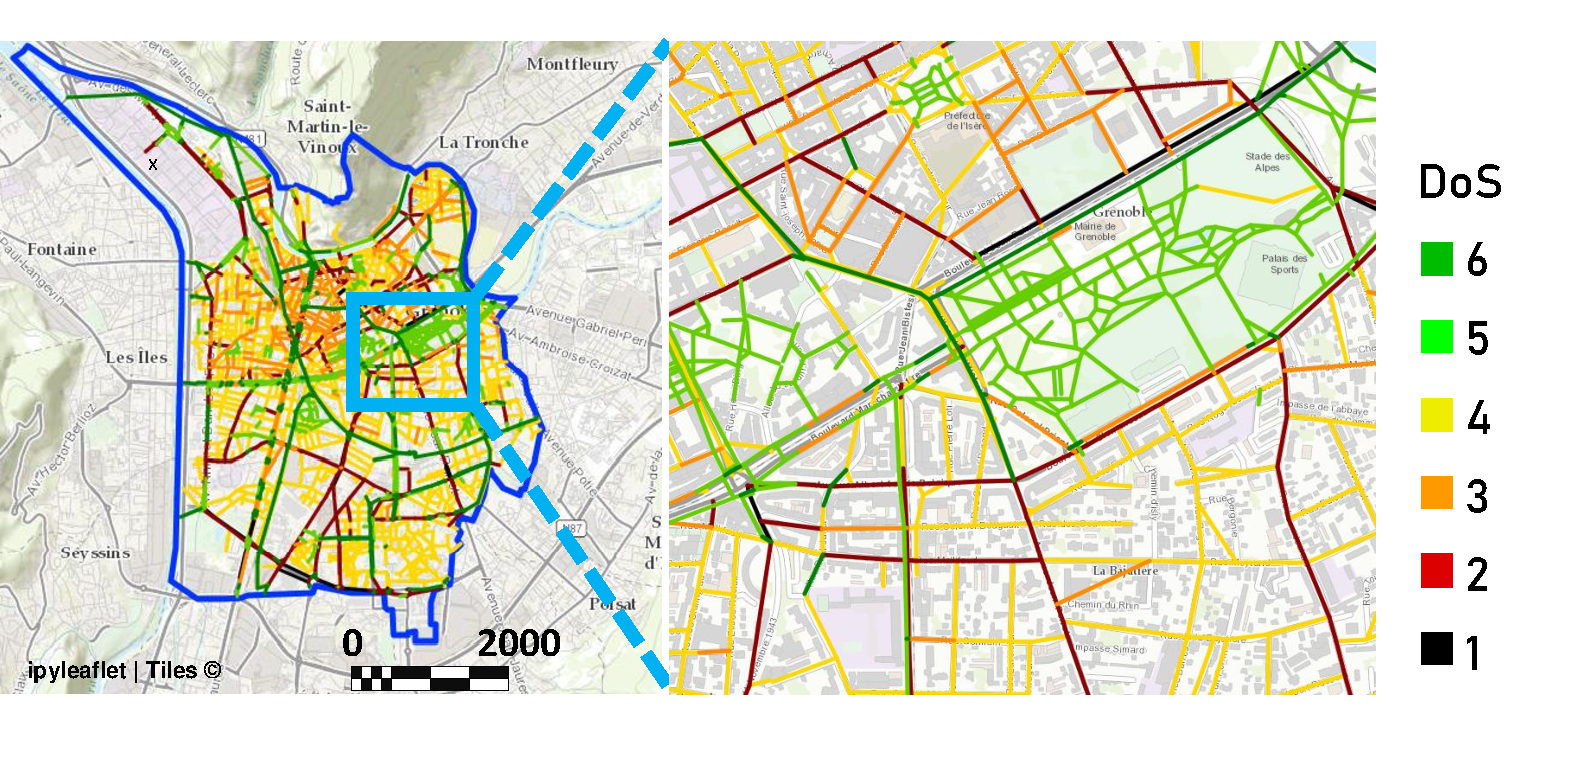
\includegraphics[width=\columnwidth]{Images/Map_and_scale.pdf}
\caption{\footnotesize Cycling network of Grenoble, France. The degree of separation (DoS) score, indicating infrastructure safety, ranges from 1 to 6.}
\label{networks_classification}
\end{figure}

\textit{Related Work:} Our work draws on two primary domains: cycling network optimization and transport justice. The following is an overview of related work in these areas.

Cycling network optimization uses diverse methodologies, including bi-level frameworks that balance cyclist distance maximization with car travel time reduction \cite{mesbah2012bilevel}, while cost-benefit analyses guide phased network expansions \cite{paulsen2023societally}. Graph-theoretic approaches prioritize low-cost connectivity \cite{duthie2014optimization}, and others optimize route efficiency under budget constraints, incorporating terrain and traffic flow predictions \cite{cooper2017using}. Recent graph-based methods focus exclusively on safety improvements \cite{2024graphbased}. However, these methods overlook the fair distribution of resources.

Transport justice proposes to design and operate transport systems in line with principles of social justice. Thereby, the seminal work by Martens~\cite{martens2017transport} argues for a sufficientarian perspective on accessibility. Which is further supported in~\cite{pereira2017distributive} to evaluate transit accessibility levels, and mobilized into a prescriptive optimization framework for intermodal transport planning in~\cite{salazar2024accessibility}.
The capabilities approach is applied in \cite{amorim2024comparing} and \cite{randal2020fairness} to emphasize minimum standards and guide policy developments which \cite{mullen2021mobility} explored through normative planning approaches.
Nevertheless, except for~\cite{salazar2024accessibility}, most of these papers are aimed at evaluation rather than prescription, and do not focus on cycling safety. 

To the best of the authors' knowledge there is no framework to optimize bicycle network safety upgrades in line with principles of justice.


% The optimization framework proposed in this paper contribute to integrate transport justice principles into cycling network design, balancing efficiency and equity. While prior studies focus on connectivity, cost, or safety, they often overlook equitable resource distribution. We address this gap by aiming to maximize cyclist safety through two principles of justice: the conventional utilitarian and the sufficientarian perspective. The bi-level framework models infrastructure planning as a two-stage process: the lower level estimates cyclist flows using all-or-nothing assignment based on slope and annual average daily traffic (AADT); the upper level optimizes upgrades to improve safety under budget constraints. We solve this problem using a budget-efficient genetic algorithm and compare it to a -based method that has been shown to effectively improve overall safety in cycling networks~\cite{2024graphbased}. Applied to Grenoble’s cycling network, our approach enhances safety for all cyclists, with particular benefits for the most vulnerable.

% In conclusion, to the best of our knowledge, transport justice principles have yet to be systematically integrated into cycling infrastructure optimization, particularly for safety, representing a significant gap in achieving fair and equitable safety improvements for all cyclists.
% The proposed optimization framework integrates transport justice principles into cycling network design by balancing efficiency and equity. Unlike prior studies that focus on connectivity, cost, or safety alone, our approach addresses the fair distribution of resources. We apply two ethical perspectives: the utilitarian, maximizing total safety, and the sufficientarian, ensuring a minimum safety threshold for most of the cyclists. The bi-level model estimates cyclist flows using an all-or-nothing assignment based on slope and traffic, and allocates upgrades under budget constraints. We solve this problem using a budget-efficient genetic algorithm and compare it to a -based method shown to improve safety~\cite{2024graphbased}. Applied to Grenoble’s cycling network, our framework enhances safety for all users, especially the most vulnerable. In conclusion, to the best of the author's knowledge, this is the first systematic application of transport justice principles to optimize cycling infrastructure with a focus on safety.

\textit{Statement of Contributions:} This work presents a bi-level optimization framework for cycling infrastructure planning to improve safety by conforming to the principle of justice. Given budget constraints, we aim to increase the degree of separation (DoS) between bike lanes and car lanes according to utilitarian and sufficientarian distribution paradigms.
We capture cyclist flows with an all-or-nothing (AON) assignment that captures slope and traffic conditions. The problems are solved using a budget-efficient genetic algorithm and are compared to a connectivity-based approach~\cite{2024graphbased}.
Applied to Grenoble’s cycling network, our framework improves safety for all users, particularly the most vulnerable.
In conclusion, we firmly believe that this is the first systematic application of transport justice principles to optimize cycling infrastructure safety upgrades.      



% \begin{table*}[t]
% \centering
% \vspace{0.2cm}
% \begin{tabular}{|>{\centering\arraybackslash}p{0.02\linewidth}|p{0.40\linewidth}|>{\centering\arraybackslash}p{0.18\linewidth}|C{0.13\linewidth}|C{0.14\linewidth}|}
% \hline
% \textbf{DoS}   & \textbf{Description} & \textbf{Geovelo} & \textbf{AADT (veh/day)} & \textbf{Mean speed (km/hr)} \\
% \hline
%  $6$ & Dedicated bike lanes, fully separated from motor traffic. & 7, 14 & 14 400 & 50 \\

% $5$  & Bike lanes shared with pedestrians, separate from cars. & 2, 10, 11, 15, 16, 17, 20 & 16 000 & 50 \\ 
% $4$  & Mixed-traffic roads (30 km/h) without designated bike lanes. & 9, 12, 13, 21, 22 & 960 & 30  \\

% $3$  & Shared roads with cycling pictograms. & 5, 8 & 3 120 & 30 \\

% $2$  & Roads with painted bike lanes. & 1, 3, 4, 6 & 6 912 & 40  \\

% $1$  & Unmarked shared car-bike lanes. & 18, 19 & 8 448 & 40  \\
% \hline



% \end{tabular}
% \caption{\footnotesize The first column represents the degree of separation (DoS), which categorizes bike lane infrastructure based on safety levels. The second column describes the category of cycling infrastructure. The third column lists the corresponding Geovelo classification numbers. The fourth and fifth columns present data from the GTLVille platform in Grenoble, detailing annual average daily traffic (AADT) and car mean speed in the adjacent roads to cycling paths, respectively.}
% \label{dos_table}
% \end{table*}

\begin{table}[t]
\centering
\vspace{0.2cm}
\begin{tabular}{|>{\centering\arraybackslash}p{0.1\linewidth}|p{0.60
\linewidth}|C{0.15\linewidth}|}
\hline
\textbf{DoS}   & \textbf{Description} & \textbf{AADT (veh/day)} \\
\hline
$6$  & Dedicated bike lanes, fully separated from motor traffic. & 14 400 \\

$5$  & Bike lanes shared with pedestrians, separate from cars. & 16 000 \\ 

$4$  & Mixed-traffic roads (30 km/h) without designated bike lanes. & 960  \\

$3$  & Shared roads with cycling pictograms. & 3 120 \\

$2$  & Roads with painted bike lanes.  & 6 912 \\

$1$  & Unmarked shared car-bike lanes. & 8 448 \\
\hline
\end{tabular}
\caption{\footnotesize The degree of separation (DoS) categorizes bike lane infrastructure based on safety levels. The third column presents annual average daily traffic (AADT) on adjacent roads, sourced from the GTLVille platform in Grenoble \cite{gtlville2024}.}
\label{dos_table}
\end{table}

\textit{Organization:} The structure of this paper is as follows: Section  \ref{model_design} discusses the data sources, bike lane classification and outlines the model design, including the flow assignment method, bi-level optimization with utilitarian and sufficientarian perspectives, and the algorithms used to solve them. Section \ref{study_case} presents a case study on the Grenoble cycling network. Finally, Section~\ref{conclusions} concludes with key findings and future research directions
%%%%%%%%%%%%%%%%%%%%%%%%%
\section{Model Design}
\label{model_design}
In this section, we first present the bike lane classification and the graph representation. Next, we introduce the cyclist flow prediction model and the bi-level optimization problems: The first adopts a utilitarian perspective to minimize cyclists' traffic exposure, directing flows toward safer routes, and reducing high-traffic exposure to improve overall safety, while the second follows a sufficientarian perspective, aiming to reduce the number of cyclists falling below relative safety thresholds. Finally, we introduce the two algorithms designed to solve these NP-hard problems.

\subsection{Bike Lane  Safety classification}

% The DoS classification, adapted from Geovelo's OSM-based platform\footnote{\url{https://gitlab.com/geovelo-public/requetes_amenagements_cyclables/-/tree/master}}, is simplified into six levels based on separation from motor traffic.  Table~\ref{dos_table} presents DoS categories, showing that higher-DoS lanes offer greater safety. These scores serve as weights for the links in the network graph and provide the framework for modeling upgrades from lower to higher safety levels. Fig.~\ref{networks_classification} visualizes these classifications in the Grenoble cycling network. The classification methodology, developed in \cite{2024graphbased}, is publicly available online\footnote{\url{https://github.com/leunamCampero/ITSC2024}}. 
The DoS classification, adapted from an OSM-based platform, categorizes cycling infrastructure based on separation from motor traffic. Table~\ref{dos_table} presents DoS categories, showing that higher-DoS lanes offer greater safety. These scores serve as weights in the network graph, modeling upgrades from lower to higher safety levels. The classification methodology is detailed in \cite{2024graphbased}. Fig.~\ref{networks_classification} visualizes these classifications in the Grenoble cycling network.

\subsection{Graph Representation}

% Let the considered network be represented by a weighted directed graph (digraph) $\mathcal{G} = (\mathcal{V}, \mathcal{A}, \mathcal{W})$, where:
% \begin{itemize}
%     \item $\mathcal{V}$ denotes the set of nodes (vertices), corresponding to intersections or road endpoints,
%     \item $\mathcal{A}$ denotes the set of directed links (arcs), representing roads, and
%     \item $\mathcal{W}$ denotes the set of weights assigned to the links.
% \end{itemize}

% For each arc $a = (u,v) \in \mathcal{A}$, where $u,v \in \mathcal{V}$ are nodes in the network, the weight $w_a \in \mathcal{W}$ represents the DoS associated with the link. The weights are symmetric, i.e., $w_{(u,v)} = w_{(v,u)}$. The geographical length of an arc $a$ is denoted by $d_a$. 
Let the network be represented by a weighted directed graph (digraph) $\mathcal{G} = (\mathcal{V}, \mathcal{A}, \mathcal{W})$, where $\mathcal{V}$ is the set of nodes corresponding to intersections or road endpoints, $\mathcal{A}$ is the set of directed arcs representing roads, and $\mathcal{W}$ is the set of weights assigned to those arcs. For each arc $a = (u, v) \in \mathcal{A}$, with $u,v \in \mathcal{V}$, the weight $w_a \in \mathcal{W}$ represents the DoS associated with the link. The weights are assumed to be symmetric, meaning $w_{(u,v)} = w_{(v,u)}$. The geographical length of each arc $a$ is denoted by $d_a$.




  
%%%%%%%%%%%%%%%%%%%%%%%%%%%%%%%%%%%%%%%%%%%%%%%%%%%%%%%%%%%%%%%%%%%%%%%%%%%%%%%%%%%%%%%%%%%%%%%%%%%%%%%%%%
\subsection{Cyclist Flows}
\label{section_flows}
%%%%%%%%%%%%%%%%%%%%%%%%%%%%%%%%%%%%%%%%%%%%%%%%%%%%%%%%%%%%%%%%%%%%%%%%%%%%%%%%%%%%%%%%%%%%%%%%%%%%%%%%%%




% Following \cite{mesbah2012bilevel}, an all-or-nothing traffic assignment model assumes no congestion, assigning all demand $q_{(u,v)}$ from the EMD2020 household survey \cite{SMMAG_EMD} to the shortest path between nodes $u$ and $v$. This reflects cycling traffic dynamics, where cyclists occupy less space and experience minimal congestion effects compared to motorized vehicles. This simplification allows for straightforward flow computation, as in \cite{cooper2017using}, where OpenStreetMap and Cardiff cycling flow data are used to define a custom distance metric incorporating infrastructure characteristics, and betweenness centrality is applied to estimate flow distribution. Based on this approach, we provide a formalized method in the following section.
Following \cite{mesbah2012bilevel}, we use an all-or-nothing (AON) traffic assignment model that assumes no congestion and assigns all demand $q_{(u,v)}$ from the EMD2020 survey \cite{SMMAG_EMD} to the shortest available path  between nodes $u,v \in \mathcal{V}$. This reflects typical cycling dynamics, where congestion effects are minimal. In this section, we formalize and adopt the cyclist distance proposed in \cite{cooper2017using}, which defines this distance using OpenStreetMap and Cardiff cycling flow data while incorporating infrastructure characteristics. Then, betweenness centrality is applied to estimate the flow distribution.

To account for cycling-specific factors, we use a modified distance metric that accounts for key factors influencing route choice. Let $\mathcal{V}$ denote the set of nodes in the network, and let $u, v \in \mathcal{V}$ be two nodes. The shortest path between $u$ and $v$ is represented as $p_{(u,v)} = (a_{1},\ldots, a_{k})$, where each arc $a~\in~p_{(u,v)}$ has a geographical length $d_{a}$, an angular change $\measuredangle_a$ (in degrees, either along $a$ or at junctions between consecutive arcs), a slope factor $s_{a}$ (which depends on the terrain slope $m_{a}$), and a traffic factor $f_{a}$ (that takes into account the flow of car traffic on roads adjacent to bike lanes). We define the cyclist distance $b_{(u,v)}$ between nodes $u$ and $v$ as

\begin{equation}
\label{cyclist_distance}
    b_{(u,v)} = \sum_{a \in p_{(u,v)}} \left( d_a \cdot s_a \cdot (f_a)^{\rho} \right) +  \sum_{a \in p_{(u,v)}} \measuredangle_a \cdot \kappa,
\end{equation}
where $\rho > 0$ and $\kappa > 0$ are calibration parameters controlling the influence of traffic conditions and angular changes, respectively.
The traffic factor $f_a$ is defined as
\begin{equation}
\label{f_a}
f_a = 
     \begin{cases}
\psi \cdot \exp{\left( x^{\text{AADT}}_{a} \right)} & \text{if } w_a < 5, \\
\psi \cdot 2.03 & \text{if } w_a = 5, \\
\psi & \text{if } w_a = 6.
\end{cases}
\end{equation}

Here, $x^{\text{AADT}}_{a}$ represents the annual average daily traffic (AADT) of the adjacent car lanes, expressed in thousands. The variable $w_a$ denotes the DoS of the bike lane $a$. According to \cite{cyclerap2024}, the impact of annual average daily traffic (AADT) is neutralized when $w_a \geq 5$, indicating full separation from car lanes. The factor 2.03 accounts for an observed increase in crash risk in shared spaces with pedestrians compared to separate, exclusive bicycle lanes \cite{mesimaki2021near}. The parameter $\psi$ is a scaling factor.  



% Let $p_{(u,v)}$ be the shortest path between nodes $u$ and $v$ using the cyclist distance in \eqref{cyclist_distance}. Then, since in our case the origin-destination (O-D) demand is symmetric, we have that each node functions both as a source and as a sink, meaning the inflow and outflow are balanced over the full cycle. The  for paths can thus be expressed as:

% \begin{equation}
% \label{eq_shortest_path}
%     x_  = q_{(u,v)},
% \end{equation}
% where $q_{(u,v)}$ is the demand from node $u$ to node $v$.

% Let $\sigma_{p_{(u,v)}}(a)$ be a binary variable indicating whether arc $a$ is part of path $p_{(u,v)}$. Then, we define  the cyclist flow on arc $a$, as

% \begin{equation}
% \label{eq_flows}
%   x_{a} = \sum_{u,v \in \mathcal{V}} q_{(u,v)} \cdot \sigma_{p_{(u,v)}}(a) \geq 0 \quad \forall a \in \mathcal{A}.
% \end{equation}

% This formulation ensures that the total flow across any arc is the sum of the demands for all trips that pass through that arc, with each node balancing its role as a source and sink due to the symmetry of the demand matrix.

Let $p_{(u,v)}$ be the shortest path between nodes $u$ and $v$ based on the cyclist distance in \eqref{cyclist_distance}. Since the origin-destination (OD) demand in our data is symmetric, each node acts as both an origin and a destination, ensuring balanced inflow and outflow. The flow conservation for paths is given by

\begin{equation}
\label{eq_shortest_path}
    x_{p_{(u,v)}} = q_{(u,v)},
\end{equation}
where $q_{(u,v)}$ represents the demand between nodes $u$ and $v$.  

Next, let $\sigma_{p_{(u,v)}}(a)$ be a binary variable indicating whether arc $a$ is part of the shortest path $p_{(u,v)}$. Then, the total cyclist flow on arc $a$, denoted as $x_a$, is

\begin{equation}
\label{eq_flows}
  x_{a} = \sum_{u,v \in \mathcal{V}} q_{(u,v)} \cdot \sigma_{p_{(u,v)}}(a) \geq 0, \quad \forall a \in \mathcal{A}.
\end{equation}
This ensures that the total flow on each arc is the sum of all demands for trips passing through it, maintaining balance across the network due to the symmetry of the demand matrix.


To assess cyclist exposure to traffic conditions, we introduce $\mathcal{E}$ as a general measure of exposure, defined for pahts in the network. This metric helps evaluate network improvements. For a shortest path $p_{(u,v)} = (a_1, \dots, a_k)$, cyclist exposure captures the combined effect of traffic-related risk and the distance of cyclist interaction with traffic, and is defined as
\begin{equation}
\label{exposure_def}
    \mathcal{E}_{p_{(u,v)}} = \sum_{a \in p_{(u,v)}} d_{a} \cdot f_{a},
\end{equation}
where $d_{a}$ and $f_{a}$ are the normalized arc length and traffic factor, respectively. For a single arc $a \in \mathcal{A}$, cyclist exposure simplifies to
\begin{equation}
\label{arc_exposure}
    \mathcal{E}_{a} = d_{a} \cdot f_{a} \in  \left [ 0,1 \right ].
\end{equation}

Next, we introduce the bi-level optimization frameworks to improve cyclist safety. The lower-level problem estimates cyclist flows via AON assignment, incorporating slope and traffic factors. The upper-level optimization selects lane upgrades to reduce cyclist exposure while incorporating both utilitarian and sufficientarian transport justice principles. Additionally, we introduce the algorithms designed to solve these problems efficiently.



%%%%%%%%%%%%%%%%%%%%%%%%%%%%%%%%%%%%%%%%%%%%%%%%%%%%%%%%%%%%%%%%%%%%%%%%%%%%%%%%%%%%%%%%%%%%%%%%%%%%%%%%%%
\subsection{Optimization Problem (Utilitarian Perspective)}
\label{optimization_problem}

Given a fixed budget $B$, we adopt a utilitarian perspective to improve cycling infrastructure by upgrading the DoS on selected road segments. The goal is to minimize cyclists’ average exposure to vehicular traffic, accounting for their flow distribution across the network. Each upgrade incurs a cost per meter and must comply with budget constraints. We define the following notations:


\begin{itemize}
    \item $\mathbf{w}_{0} = \left [ w_{1}, \ldots, w_{a}, \ldots, w_{|\mathcal{A}|} \right ]^\top \in \mathbb{N}^{|\mathcal{A}|}$: the original arc weights (DoS) of the graph $\mathcal{G}$;
    \item $\tilde{\mathbf{w}} = \left [ \tilde{w}_{1}, \ldots, \tilde{w}_{a}, \ldots, \tilde{w}_{|\mathcal{A}|} \right ]^\top \in \Omega$: the candidate weights to be optimized, whereby
\end{itemize}

\begin{equation}
\Omega = \left \{ \tilde{w} \in \mathbb{N}^{|\mathcal{A}|} \colon w_{a} \leq \tilde{w}_{a} \leq 6,  \forall a \in \{1, \ldots, |\mathcal{A}| \} \right\};    
\end{equation}

Additionally, we define the following, where the values are normalized to be scaled between their respective minimum and maximum values:

\begin{itemize}
    \item $\mathbf{b}(\tilde{\mathbf{w}}) = \left [ b_{1}, \cdots, b_{a}, \cdots, b_{|\mathcal{A}|} \right ]^\top \in \mathbb{R}^{|\mathcal{A}|}_{\geq 0}$: the vector of normalized  cyclist distances, defined in~\eqref{cyclist_distance};
    \item $\mathbf{x}^\star(\tilde{\mathbf{w}}) = \left [ x_{1}, \cdots, x_{a}, \cdots, x_{|\mathcal{A}|} \right ]^\top \in \mathbb{R}^{|\mathcal{A}|}_{\geq 0}$: the vector of normalized arc flows resulting from the AON assignment, computed according to~\eqref{eq_shortest_path} and~\eqref{eq_flows};
    \item $\boldsymbol{\mathcal{E}}(\tilde{\mathbf{w}}) = \left [ \mathcal{E}_{1}, \cdots, \mathcal{E}_{a}, \cdots, \mathcal{E}_{|\mathcal{A}|} \right ]^\top \in \mathbb{R}^{|\mathcal{A}|}_{\geq 0}$: the vector of traffic exposure, which is also a function of the chosen upgrades $\tilde{\mathbf{w}}$, as defined in~\eqref{arc_exposure};
    \item $\pi(w_{a},\tilde{w}_{a}) \in \mathbb{R}_{\geq 0}$: the cost per meter of upgrading arc $a$ from its original DoS $w_{a}$ to the new DoS $\tilde{w}_{a}$;
    \item $J_{\mathcal{E}} = \boldsymbol{\mathcal{E}}^\top(\tilde{\mathbf{w}}) \mathbf{x}^\star(\tilde{\mathbf{w}}) \in \mathbb{R}_{\geq 0}$: the total cyclist exposure throughout the network, where both $\boldsymbol{\mathcal{E}}$ and $\mathbf{x}^{\star}$ depend on the chosen DoS levels $\tilde{\mathbf{w}}$.
    %This objective corresponds to the utilitarian perspective, as it aims to maximize overall safety improvements across the network. 
\end{itemize}
We formulate the problem as a bi-level optimization, where the upper level selects infrastructure upgrades and the lower level determines cyclist route choices based on the resulting network.

\textit{Upper-Level Problem} ($\mathbb{U}$): This attempts to minimize cyclist exposure to car traffic by selecting optimal DoS upgrades while respecting budget $B$. The objective function prioritizes upgrades on long arcs with high traffic and cyclist flow, as these segments pose the greatest safety risks.

\textit{Lower-Level Problem} ($\mathbb{L}$): It aims to model cyclist flow distribution after the upgrades. It assigns each OD pair to the shortest cyclist-distance path using an AON assignment, as described in Section~\ref{section_flows}, ensuring that the flow distribution reflects route safety.




Since changes in DoS affect both the perceived cyclist distance and the resulting flow distribution, the two levels are nested: Decisions in the upper level directly influence the lower-level solution.

% \begin{problem}[Utilitarian Network-Upgrade]
% \label{utilitarian_problem}
% \begin{align}
% \mathbb{P}_{1}: \quad  \, &  \mathbf{w}^{\star}  = \arg\min_{\tilde{\mathbf{w}} \in \Omega} \;  J_{\text{util}} (\tilde{\mathbf{w}})  \\ 
% \text{s.t. } &   \sum_{a=1}^{|\mathcal{A}|} d_{a} \cdot \pi(w_{a},\tilde{w}_{a})  \leq B  \label{budget_constraint} \\
% \mathbb{P}_{2}: \quad  \, &  \mathbf{x}^{\star}(\tilde{\mathbf{w}})   = \arg\min_{\mathbf{x} \in \mathbb{R}^{|\mathcal{A}|}_{\geq 0}} \; \mathbf{b}(\tilde{\mathbf{w}})^\top \mathbf{x} \label{eq_utilitarian_obj} \\
% \text{s.t. }  & \quad x_{p} = q, \quad x_a = \sum q \cdot \sigma_{p}(a) \geq 0 \label{eq_utilitarian_constraints} \\
% & \quad \text{as in \eqref{eq_shortest_path} and \eqref{eq_flows}}. \nonumber
% \end{align} 
% \end{problem}
\begin{problem}[Utilitarian Network-Upgrade]
\label{utilitarian_problem}
\begin{align}
\mathbb{U}: \quad  \, &  \mathbf{w}^{\star}  = \arg\min_{\tilde{\mathbf{w}} \in \Omega} \;  J_{\mathcal{E}} (\tilde{\mathbf{w}})  = \boldsymbol{\mathcal{E}}^\top(\tilde{\mathbf{w}}) \mathbf{x}^\star(\tilde{\mathbf{w}})\\
\text{s.t. } & \sum_{a=1}^{|\mathcal{A}|} d_{a} \cdot \pi(w_{a},\tilde{w}_{a}) \leq B \label{budget_constraint} \\
\mathbb{L}: \quad \, & \mathbf{x}^\star(\tilde{\mathbf{w}}) = \arg\min_{\mathbf{x} \in \mathbb{R}^{|\mathcal{A}|}_{\geq 0}} \; \mathbf{b}(\tilde{\mathbf{w}})^\top \mathbf{x} \label{eq_utilitarian_obj} \\
\text{s.t. }  & x_a = \sum q \cdot \sigma(a) \geq 0  \quad \forall a \in \left \{ 1,\dots, |\mathcal{A}| \right   \}  \label{eq_utilitarian_constraints} \\
& \text{as in \eqref{eq_flows}}. \nonumber
\end{align}
\end{problem}
The bi-level optimization Problem 1 is NP-hard as it requires selecting a subset of arc upgrades within a fixed budget, similar to the 0-1 knapsack problem. The challenge lies in balancing the upgrades' costs and their impact on safety, which requires combinatorial selection and may be computationally intractable for large instances. While $\mathbb{U}$ is non-convex and non-linear, $\mathbb{L}$ remains linear and convex (see Appendix~A for details).


\subsection{Optimization Problem (Sufficientarian Perspective)}
\label{section_safety_metric}
%%%%%%%%%%%%%%%%%%%%%%%%%%%%%%%%%%%%%%%%%%%%%%%%%%%%%%%%%%%%%%%%%%%%%%%%%%%%%%%%%%%%%%%%%%%%%%%%%%%%%%%%%%

Now, we incorporate a sufficientarian perspective into Problem~1 by ensuring that as many individuals as possible achieve a minimum level of safety on paths throughout the network. Using the definition of path exposure $\mathcal{E}_{p_{(u,v)}}$ from \eqref{exposure_def}, we define the safety score of a path as
\begin{equation}
    s_{p_{(u,v)}} = \frac{1}{\mathcal{E}_{p_{(u,v)}} + \epsilon},
\end{equation}
where $\epsilon > 0$ avoids division by zero and limits the maximum safety score. This score reflects the inverse relationship between cyclist exposure and perceived safety, consistent with established findings in route choice modeling \cite{casello2014modeling}, where cyclists prefer routes with lower traffic volumes. Although this formulation is a simplification, it serves as a continuous proxy for perceived safety when only exposure data is available. 

To determine what constitutes a sufficient level of safety, we adopt a relative threshold approach. Let the global average safety across all regions be
\begin{equation}
    s_{\mathcal{G}} = \frac{1}{|\mathcal{V}|} \sum_{u \in \mathcal{V}} s_{p_{(u,v)}} \quad \forall v \in \mathcal{V}.
\end{equation}
% We then define the safety threshold $s_{\text{thr}}$ as a proportion of this average:
% \begin{equation}
%     s_{\text{thr}} = \lambda s_{\mathcal{G}},
% \end{equation}
% $\lambda \in \{10\%, 20\%, 30\%, 40\%, 50\%\}$ represents a set of relative thresholds. This method follows the standard practice proposed by Martens in the context of transport justice~\cite{martens2017transport, martens2022equity}, where sufficiency thresholds are defined as a proportion of an average (or median) accessibility level.
We then define a relative safety threshold $s_{\text{thr}}$ as a proportion of the average safety level $s_{\mathcal{G}}$, using a parameter $\lambda$ that takes values from the set $\{10\%, 20\%, 30\%, 40\%, 50\%\}$.
\begin{equation}
    s_{\text{thr}} = \lambda s_{\mathcal{G}}.
\end{equation}
This method follows the standard practice proposed by Martens in the context of transport justice~\cite{martens2017transport, martens2022equity}, where sufficiency thresholds are defined as a proportion of an average (or median) accessibility level.


Cycle paths whose safety scores fall below this threshold are considered insufficiently protected. To quantify this, and following a similar approach to~\cite{salazar2024accessibility}, we define the path-level safety insufficiency as
\begin{equation}
    \mathcal{I}_{p_{(u,v)}} = \max{\left \{0,  \frac{s_{\text{thr}} - s_{p_{(u,v)}}}{s_{\text{thr}}} \right \}}.
\end{equation}
Dividing the network into regions $\mathcal{R} = \{1, \dots, R\}$, where $\mathcal{V}^{r} \subseteq \mathcal{V}$ represents nodes in region $r$, allows for regional analysis, then, the regional safety insufficiency is computed as the demand-weighted average safety insufficiency for each OD pair within the region
\begin{equation}
    \mathcal{I}_{r} = \frac{\sum_{u \in \mathcal{V}^{r}} \mathcal{I}_{p_{(u,v)}} \cdot q_{(u,v)}}{\sum_{u \in \mathcal{V}^{r}} q_{(u,v)}} \quad \forall v \in \mathcal{V},
\end{equation}
where $q_{(u,v)}$ is the demand for OD pair $(u,v)$. The total population-weighted safety insufficiency across the network is given by
\begin{equation}
    J_{\mathcal{I}} = \frac{\sum_{r \in \mathcal{R}} n_{r} \cdot \mathcal{I}_{r}}{\sum_{r \in \mathcal{R}} n_{r}},
\end{equation}
where $n_{r}$ represents the number of cyclists in region $r$. Finally, we define the sufficientarian bi-level optimization problem, where $\mathbb{U}_{\text{thr}}$ ensures that as many cyclists as possible meet the minimum relative safety threshold while minimizing cyclist exposure, and as before, $\mathbb{L}$ models the resulting flow distribution. 
%Note that although the objective is to minimize safety insufficiency, we use the subscript “suff” to emphasize the sufficientarian nature of the objective, in contrast to the fully utilitarian approach. 





\begin{problem}[Sufficientarian Network-Upgrade]  
\begin{align}
& \mathbb{U}_{\text{thr}}: \quad  \,  \mathbf{w}^{\star}  = \arg\min_{\tilde{\mathbf{w}} \in \Omega} \; \left (  J_{\mathcal{I}}(\tilde{\mathbf{w}}) + \eta \cdot J_{\mathcal{E}} (\tilde{\mathbf{w}})   \right ) \\ 
& \quad \quad  \text{s.t. }   \sum_{a=1}^{|\mathcal{A}|} d_{a} \cdot \pi(w_{a},\tilde{w}_{a})  \leq B,  \nonumber \\
& \mathbb{L}: \quad \,  \mathbf{x}^\star(\tilde{\mathbf{w}}) = \arg\min_{\mathbf{x} \in \mathbb{R}^{|\mathcal{A}|}_{\geq 0}} \; \mathbf{b}(\tilde{\mathbf{w}})^\top \mathbf{x} \label{eq_utilitarian_obj} \\
& \quad \quad  \text{s.t. }   x_a = \sum q \cdot \sigma(a) \geq 0  \quad \forall a \in \left \{ 1,\dots, |\mathcal{A}| \right   \}  \label{eq_utilitarian_constraints} \\
& \quad \quad  \quad \quad  \text{as in \eqref{eq_flows}}. \nonumber
\end{align}
\end{problem}
where $\eta$ is the regularization weight. The problem $\mathbb{U}_{\text{thr}}$ is non-convex and non-linear, analogous to its respective counterpart $\mathbb{U}$. A summary of the model notation is given in Table~\ref{table:notation_summary}.

\begin{table}[h!]
\centering
\vspace{0.2cm}
\begin{tabular}{|c|l|c|c|}
\hline
\textbf{Symbol} & \textbf{Description} & \textbf{Domain} & \textbf{Unit} \\ \hline
$q_{(u,v)}$ & Bike demand from $u$ to $v$ & $\mathbb{R}_{\geq 0}$ & bike/day \\
$p_{(u,v)}$ & Shortest path between $u$ and $v$ & $\mathcal{A}$ & - \\ 
$d_{a}$ & Arc $a$ length/distance & $\mathbb{R}_{>0}$ & m \\ 
$\measuredangle_{a}$ & Angular change at $a$ & $\mathbb{R}_{\geq 0}$ & deg \\ 
$s_{a}$ & Slope factor of arc $a$ & $\mathbb{R}_{\geq 0}$ & - \\ 
$f_{a}$ & Traffic factor on arc $a$ & $\mathbb{R}_{\geq 0}$ & - \\ 
$b_{(u,v)}$ & Cyclist distance $u$-$v$ & $\mathbb{R}_{\geq 0}$ & m \\ 
$x_{a}$ & Flow on arc $a$ & $\mathbb{R}_{\geq 0}$ & bike/day \\ 
$x_{p}$ & Flow on path $p$ & $\mathbb{R}_{\geq 0}$ & bike/day \\ 
$\sigma_{p_{(u,v)}}(a)$ & arc $a$ is part of shortest path $p$? & $ \left\{ 0,1\right\}$ & - \\ 
$\rho, \kappa, \psi$ & Calibration parameters & $\mathbb{R}$ & - \\ 
$x^{\text{AADT}}_{a}$ & AADT adjacent to $a$ & $\mathbb{R}_{\geq 0}$ & veh/day \\ 
$s_{\text{thr}}$ & safety threshold & $\mathbb{R}_{\geq 0}$ & - \\ 
$w_{a}$ & Original DoS of $a$ & $\mathbb{R}_{\geq 0}$ & - \\ 
$\tilde{w}_{a}$ & Candidate DoS for $a$ & $\mathbb{R}_{\geq 0}$ & - \\ 
$\pi(w_{a},\tilde{w}_{a})$ & Upgrade cost for $a$ & $\mathbb{R}_{\geq 0}$ & € \\ 
$\mathcal{I}_{r}$ & Regional safety insufficiency & $\mathbb{R}_{\geq 0}$ & - \\ 
$J_{\mathcal{E}}$ & Total cyclist exposure & $\mathbb{R}_{\geq 0}$ & -\\
$J_{\mathcal{I}}$ & Total safety insufficiency & $\mathbb{R}_{\geq 0}$ & - \\ 
\hline
\end{tabular}
\caption{\footnotesize Abbreviated notation for variables in cycling network model.}
\label{table:notation_summary}
\end{table}


\subsection{Solution Algorithms} 

To address the computational complexity of Problems~1 and~2, we propose two heuristic algorithms. The first is a genetic algorithm (GA) with efficient budget spending, implemented in two variants that differ only in their objective functions: \mbox{GA-U}  (Utilitarian) and \mbox{GA-S}  (Sufficientarian). As a benchmark of efficiency, we include the maximize largest connected component algorithm (MLCC) from~\cite{2024graphbased}, which enhances network connectivity by forming high-safety ($\text{DoS}~=~6$) subnetworks.




\subsubsection{Genetic Algorithm with Efficient Budget Spending ($GA$)}
The \mbox{GA-U} and \mbox{GA-S}  algorithms explore upgrade configurations under a fixed budget using a heuristic genetic approach. First, an initial population of upgrade solutions is generated and evaluated. Then, solutions are recombined (crossover) and modified (mutation) across iterations. If any budget remains, additional upgrades are greedily applied to the lowest DoS arcs. While this approach ensures efficient budget use, it may find local rather than global optima. Given the complexity of the bi-level problem, it provides feasible solutions within a reasonable time.

The pseudocode below outlines the common procedure shared by both \mbox{GA-U} and \mbox{GA-S}. The only difference lies in the objective function used to evaluate solutions: \mbox{GA-U} minimizes total cyclist traffic exposure (Problem~1), while \mbox{GA-S}  seeks to ensure that as many cyclists as possible meet a minimum safety threshold (Problem~2).

\begin{itemize}
    \item $\tilde{B}$: Remaining budget after the initial solution $\tilde{\mathbf{w}}$ has been evaluated.
    \item $\Delta_a$: Cost to upgrade arc $a$ to DoS $=6$, i.e., $\pi(\tilde{w}_a, 6)$.
\end{itemize}

\begin{algorithm}[H]
\caption{$GA$ Algorithm (used for \mbox{GA-U} and \mbox{GA-S})}
\label{pseudocode:GA}
\footnotesize
\begin{algorithmic}[1]
\State \textbf{Input:} Remaining budget $\tilde{B}$, candidate weights $\tilde{\mathbf{w}}$
\State \textbf{Output:} Updated weights $\tilde{w}_a$, remaining budget $\tilde{B}$
\For{$a \in \mathcal{A}$ sorted by $\text{DoS}(w_a)$}
    \State Compute upgrade cost: $\Delta_a = \pi(\tilde{w}_a, 6)$
    \If{$\tilde{B} \geq \Delta_a$}
        \State Upgrade $\tilde{w}_a$ to DoS $=6$
        \State Update budget: $\tilde{B} \gets \tilde{B} - \Delta_a$
    \EndIf
    \If{$\tilde{B} \leq 0$} \textbf{Exit} \EndIf
\EndFor
\State \textbf{Return:} $\tilde{w}_a$, $\tilde{B}$
\end{algorithmic}
\end{algorithm}


\subsubsection{Maximize Largest Connected Component Algorithm (MLCC)}
The MLCC algorithm \cite{2024graphbased} enhances network connectivity by strategically upgrading arcs to the highest DoS level within the budget. First, it identifies the largest connected component (CC) with DoS $=6$. Then, it connects other high DoS CCs to this primary network using the shortest path, prioritizing arcs with higher DoS values. Finally, it upgrades arcs along the path and within the CCs to DoS $=6$, iterating until the budget is exhausted. This algorithm indirectly influences cyclist flows by creating high-DoS paths. The pseudocode is outlined below, where we use the following notation:
\begin{itemize}
    \item $\mathcal{C}$: Largest connected sub-network with DoS $=6$.
    \item $\mathcal{C}_{\gamma}$: CC with DoS level $\gamma \leq 6$.
\end{itemize}

\begin{algorithm}[H]
\caption{MLCC Algorithm}
\label{pseudocode:MLCC}
\footnotesize
\begin{algorithmic}[1]
\State \textbf{Input:} Budget $B$, graph $\mathcal{G}$
\State \textbf{Output:} Upgraded DoS levels for arcs $\mathcal{A}$
\While{$B > 0$ and $\exists$ connected component $\mathcal{C}_{\gamma}$ with DoS $\gamma \leq 6$}
    \State Find shortest path between $\mathcal{C}$ and $\mathcal{C}_{\gamma}$
    \State Upgrade arcs along path to DoS $=6$ and update $B$
    \State Upgrade arcs in $\mathcal{C}_{\gamma}$ to DoS $=6$ and extend $\mathcal{C}$
\EndWhile
\State \textbf{Return:} Final DoS levels for all arcs in $\mathcal{A}$
\end{algorithmic}
\end{algorithm}

% The solution is denoted as $\mathbf{w}^{\star}_{MLCC}$.


\section{Grenoble Cycling Network Case Study}
\label{study_case}
This section introduces the parameters for the AON flow assignment, a sensitivity analysis for budget selection, and a case study of Grenoble, France. It also examines the results obtained using the MLCC, \mbox{GA-U} and \mbox{GA-S} algorithms in comparison to the original scenario.
 \subsection{Parameters and Algorithm Comparisons}
To solve the AON traffic assignment problem and determine cyclist flows, as described in Section~\ref{section_flows}, we use parameters that are better suited for the model, as suggested by \cite{cooper2017using}. Specifically, we set $\rho = 0.04$, $\kappa = 0.14$, and $\psi~=~0.84$. 

The slope factor $s_{a}$ is determined in Table~\ref{table:slope_factors}, where downhill routes are considered the reciprocal of the slope factor when traversing in the opposite direction.
\begin{table}[h!]
\centering
\begin{tabular}{c|c|c}
\hline
Slope ($m_a$) \% & Uphill Factor ($s_a$) & Downhill Factor ($s_a$) \\ \hline
$m_a < 2$ & 1.0 & 1.0 \\ 
$2 \leq m_a < 4$ & 1.371 & $1/1.371 \approx 0.729$ \\ 
$4 \leq m_a < 6$ & 2.203 & $1/2.203 \approx 0.454$ \\ 
$m_a \geq 6$ & 4.239 & $1/4.239 \approx 0.236$ \\ \hline
\end{tabular}
\caption{\footnotesize Slope factors for cycling distance calculation.}
\label{table:slope_factors}
\end{table}




\subsection{Sensitivity Analysis for Budget}
\label{budget_analysis}
 Let $B_{\text{max}}$ represent the budget required to upgrade the entire network to DoS $=6$. The cost per meter of upgrading an arc depends on the current and target DoS levels, following proportional construction costs from Cerema studies~\cite{cerema2024_cost}. The cost per meter $\pi(w_a, \tilde{w}_a)$ of upgrading arc $a$ from $w_a$ to $\tilde{w}_a$ is given by the matrix below. The total cost of upgrading an arc is computed as $d_a \cdot \pi(w_a, \tilde{w}_a)$, where $d_a$ is the arc length, making the cost distance-dependent.



\renewcommand{\arraystretch}{0.8} % Reduce row height
\setlength{\tabcolsep}{3pt} % Reduce column spacing
\begin{equation}
  \Pi =
  \scriptsize
  \begin{pmatrix} % Brackets like pmatrix
    w_{a} \textbackslash \tilde{w}_{a} & 1 & 2 & 3 & 4 & 5 & 6 \\ \hline
    1 \quad      \vert & 0\text{€}   & 150\text{€}  & 250\text{€}  & 300\text{€}  & 500\text{€}  & 750\text{€}  \\
    2 \quad   \vert & 0\text{€}   & 0\text{€}    & 100\text{€}  & 150\text{€}  & 350\text{€}  & 600\text{€}  \\
    3 \quad  \vert & 0\text{€}   & 0\text{€}    & 0\text{€}    & 50\text{€}   & 250\text{€}  & 500\text{€}  \\
    4 \quad  \vert & 0\text{€}   & 0\text{€}    & 0\text{€}    & 0\text{€}    & 200\text{€}  & 450\text{€}  \\
    5 \quad  \vert & 0\text{€}   & 0\text{€}    & 0\text{€}    & 0\text{€}    & 0\text{€}    & 250\text{€}  \\
    6 \quad \vert& 0\text{€}   & 0\text{€}    & 0\text{€}    & 0\text{€}    & 0\text{€}    & 0\text{€}    \\
  \end{pmatrix}
\end{equation}
% Instead of uniformly sampling budgets, we use a logarithmic sampling strategy that prioritizes lower budgets where significant improvements are likely. Budget ranges are defined as:
 Instead of uniformly sampling budgets, we use a logarithmic sampling strategy that prioritizes lower budgets, where significant improvements are more likely, since early investments typically target the most critical and cost-effective upgrades. Budget ranges are defined as
\begin{figure}[t]
\vspace{0.2cm}
\centering
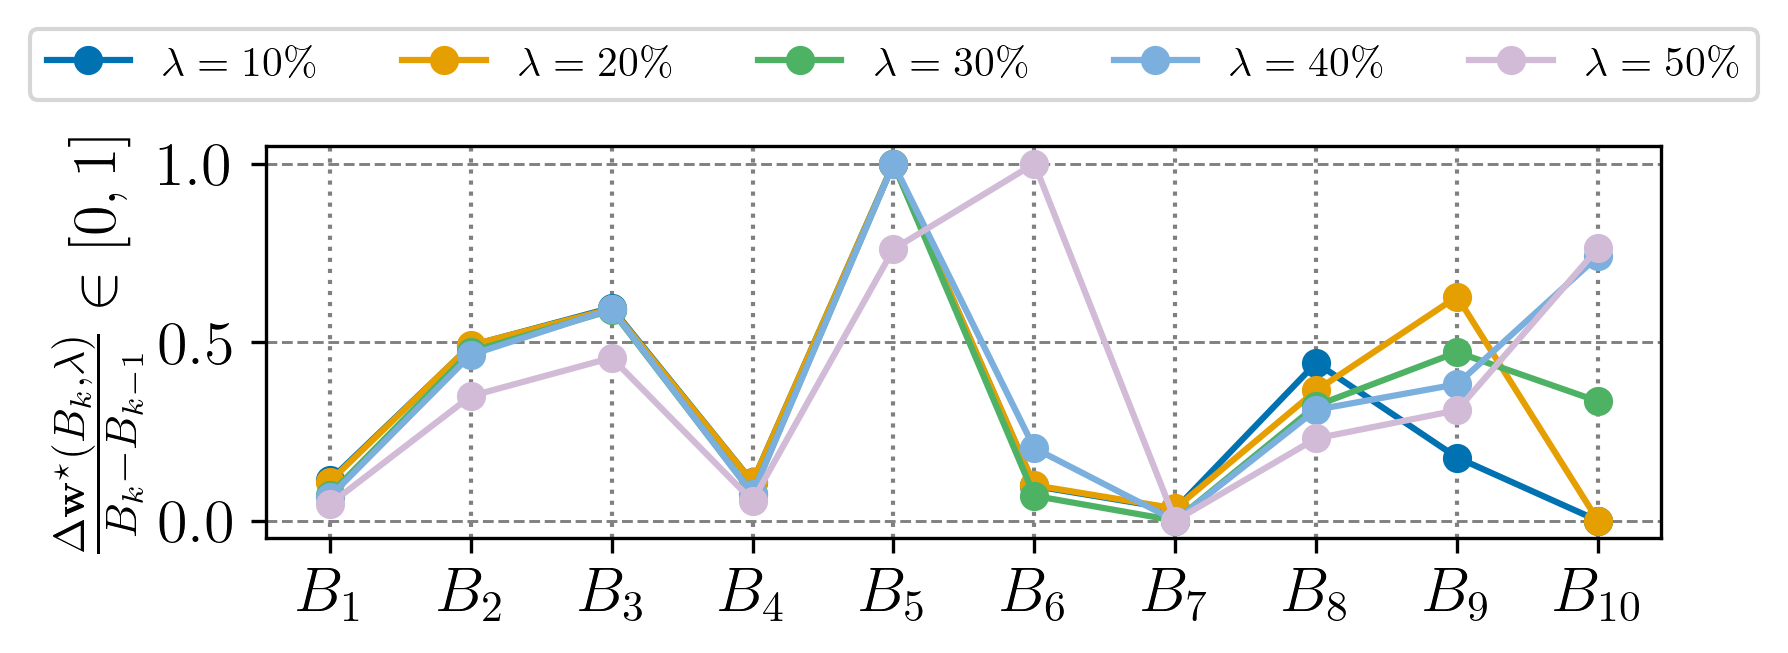
\includegraphics[width=\columnwidth]{Images/Marginal_improvements.png}
\caption{\footnotesize Normalized marginal improvements relative to budget increments to solve \eqref{marginal}.}
\label{marginal_plot}
\end{figure}
\begin{figure*}[t]
\vspace{0.2cm}
  \centering
  \captionsetup[subfigure]{font={footnotesize}, labelfont={footnotesize, bf}, textfont={footnotesize, rm}}

  \subfloat[Original DoS]{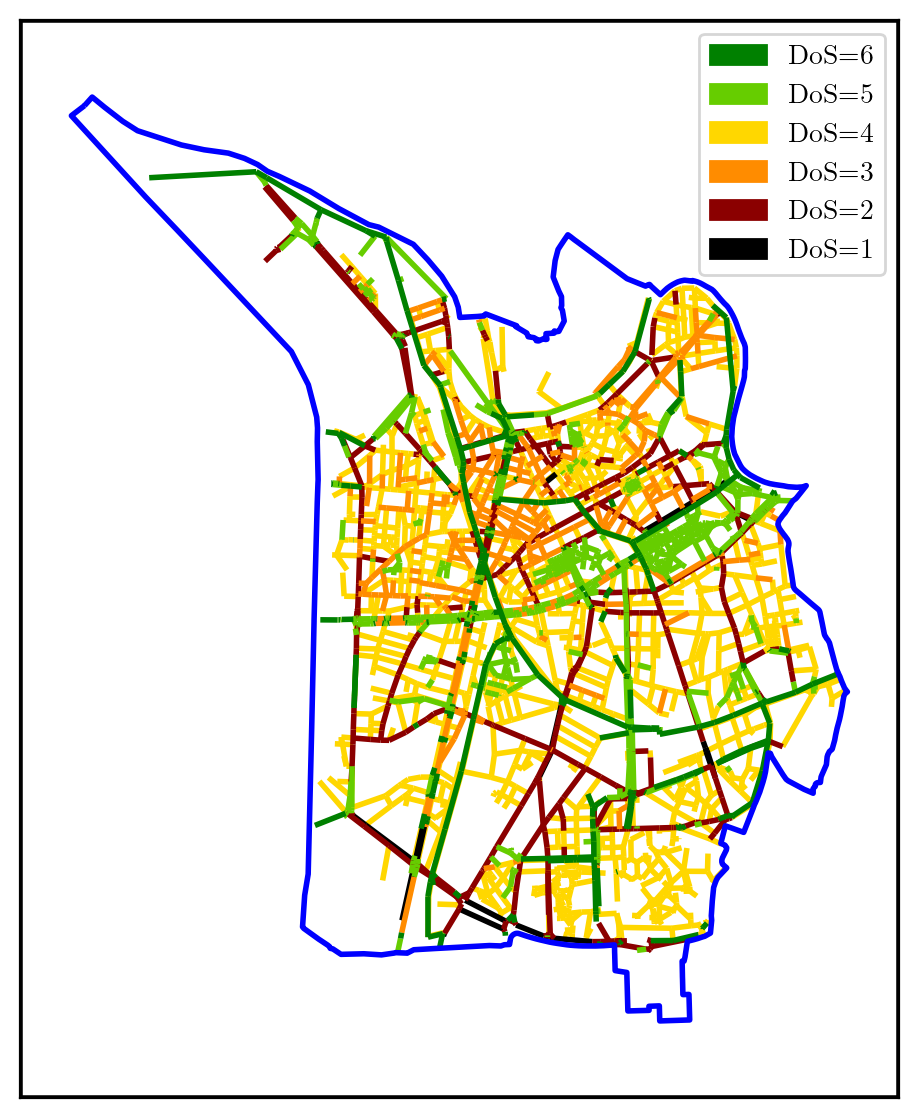
\includegraphics[width=0.23\linewidth]{Images/G_original_DoS_3.png}\label{l_2_5_1}}
  \hspace{0.012\linewidth} % Adjust horizontal space as 
  \subfloat[MLCC DoS]
  {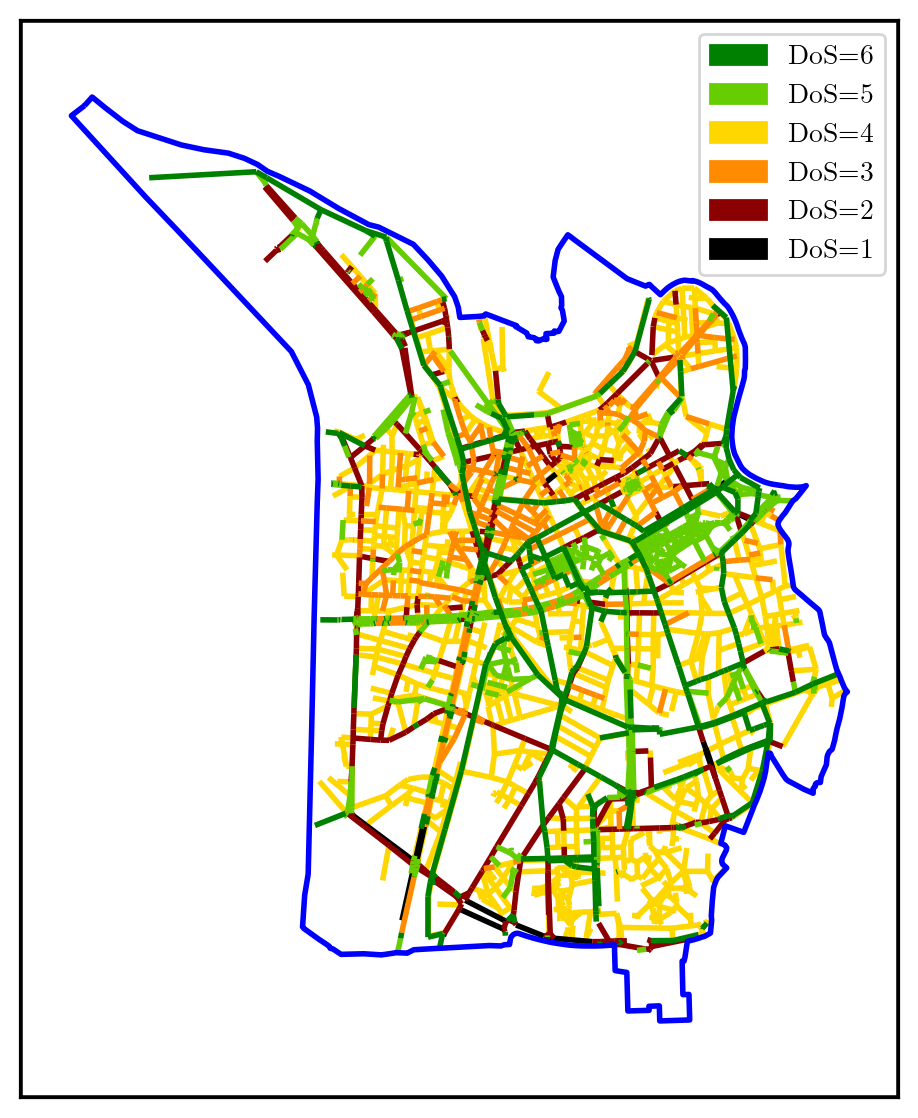
\includegraphics[width=0.23\linewidth]{Images/MLCC_DoS_3.png}\label{l_2_5_11}}
  \hspace{0.012\linewidth}
  \subfloat[\mbox{GA-U} DoS]
  {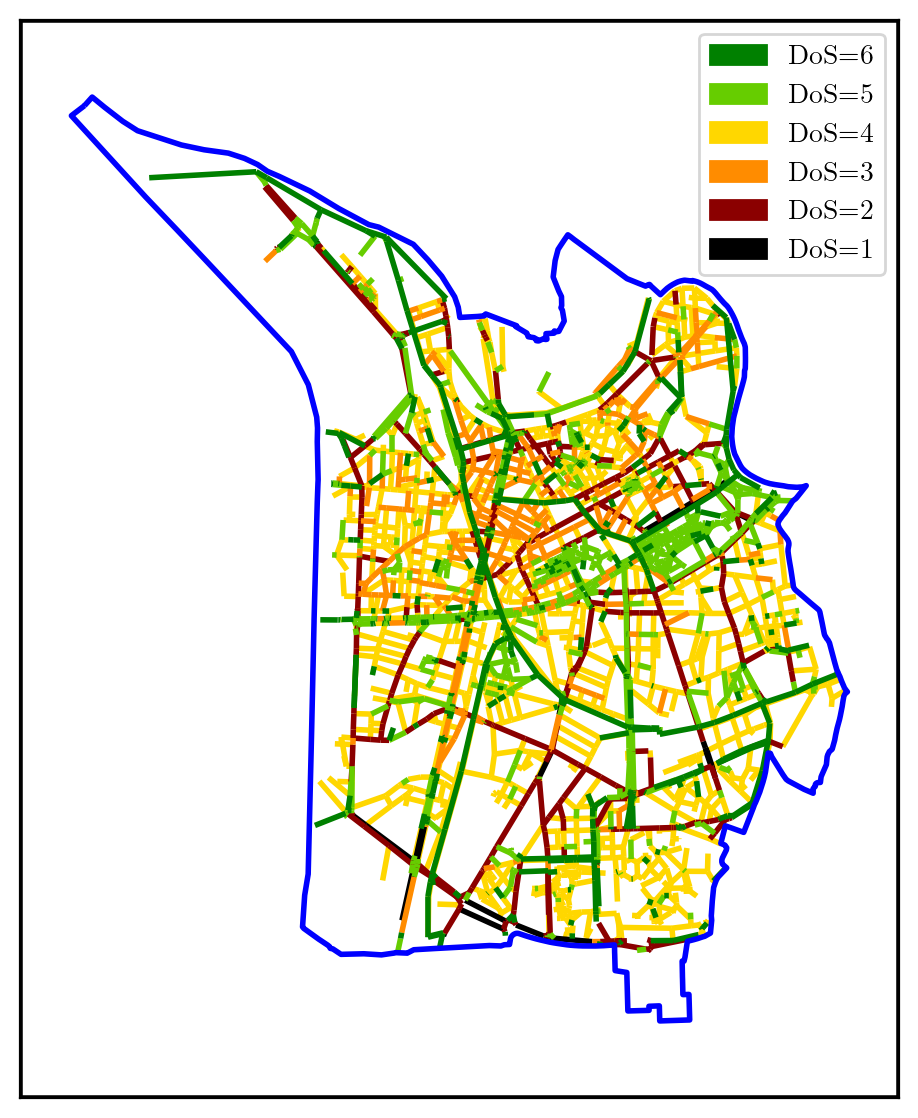
\includegraphics[width=0.23\linewidth]{Images/GAB_DoS_3.png}\label{l_2_5_2}}
  \hspace{0.012\linewidth}
  \subfloat[\mbox{GA-S} DoS]
  {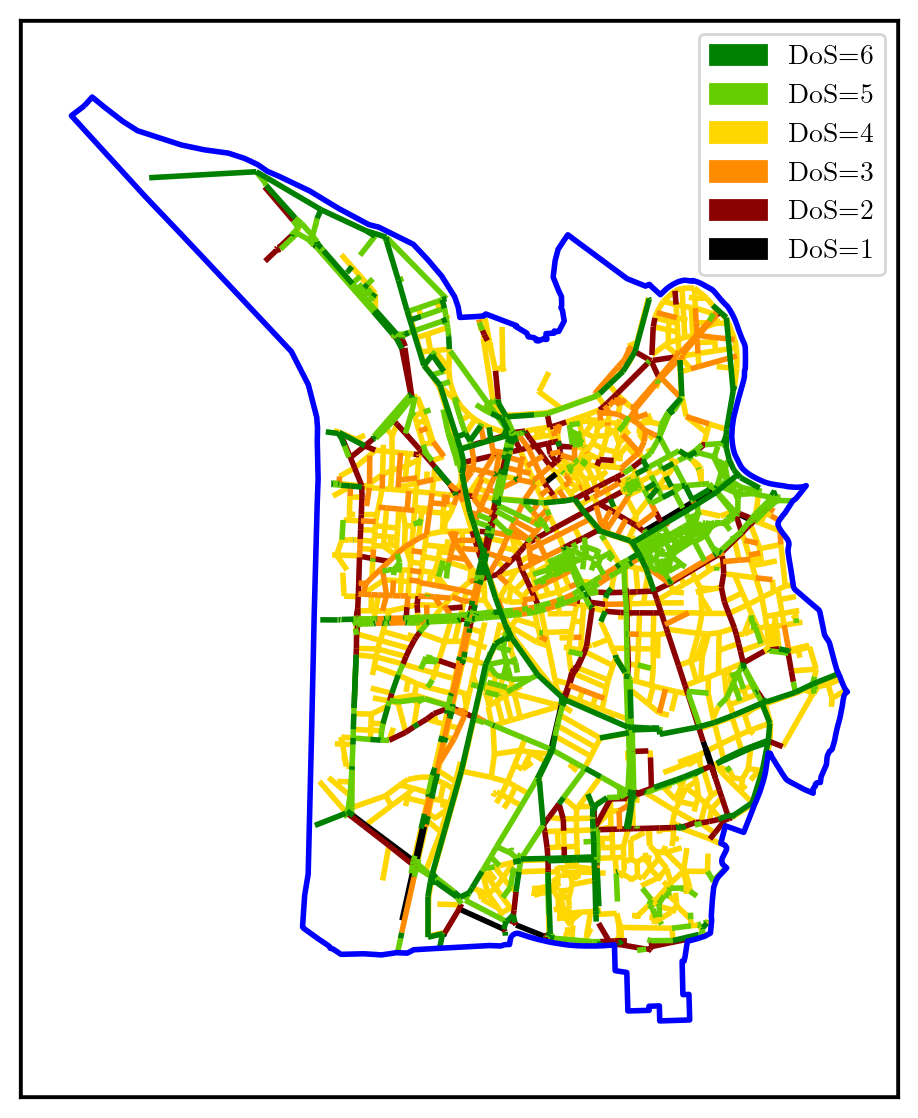
\includegraphics[width=0.23\linewidth]{Images/G_test_fair_3.png}\label{l_2_5_3}}\\
  % \subfloat[Original flow]{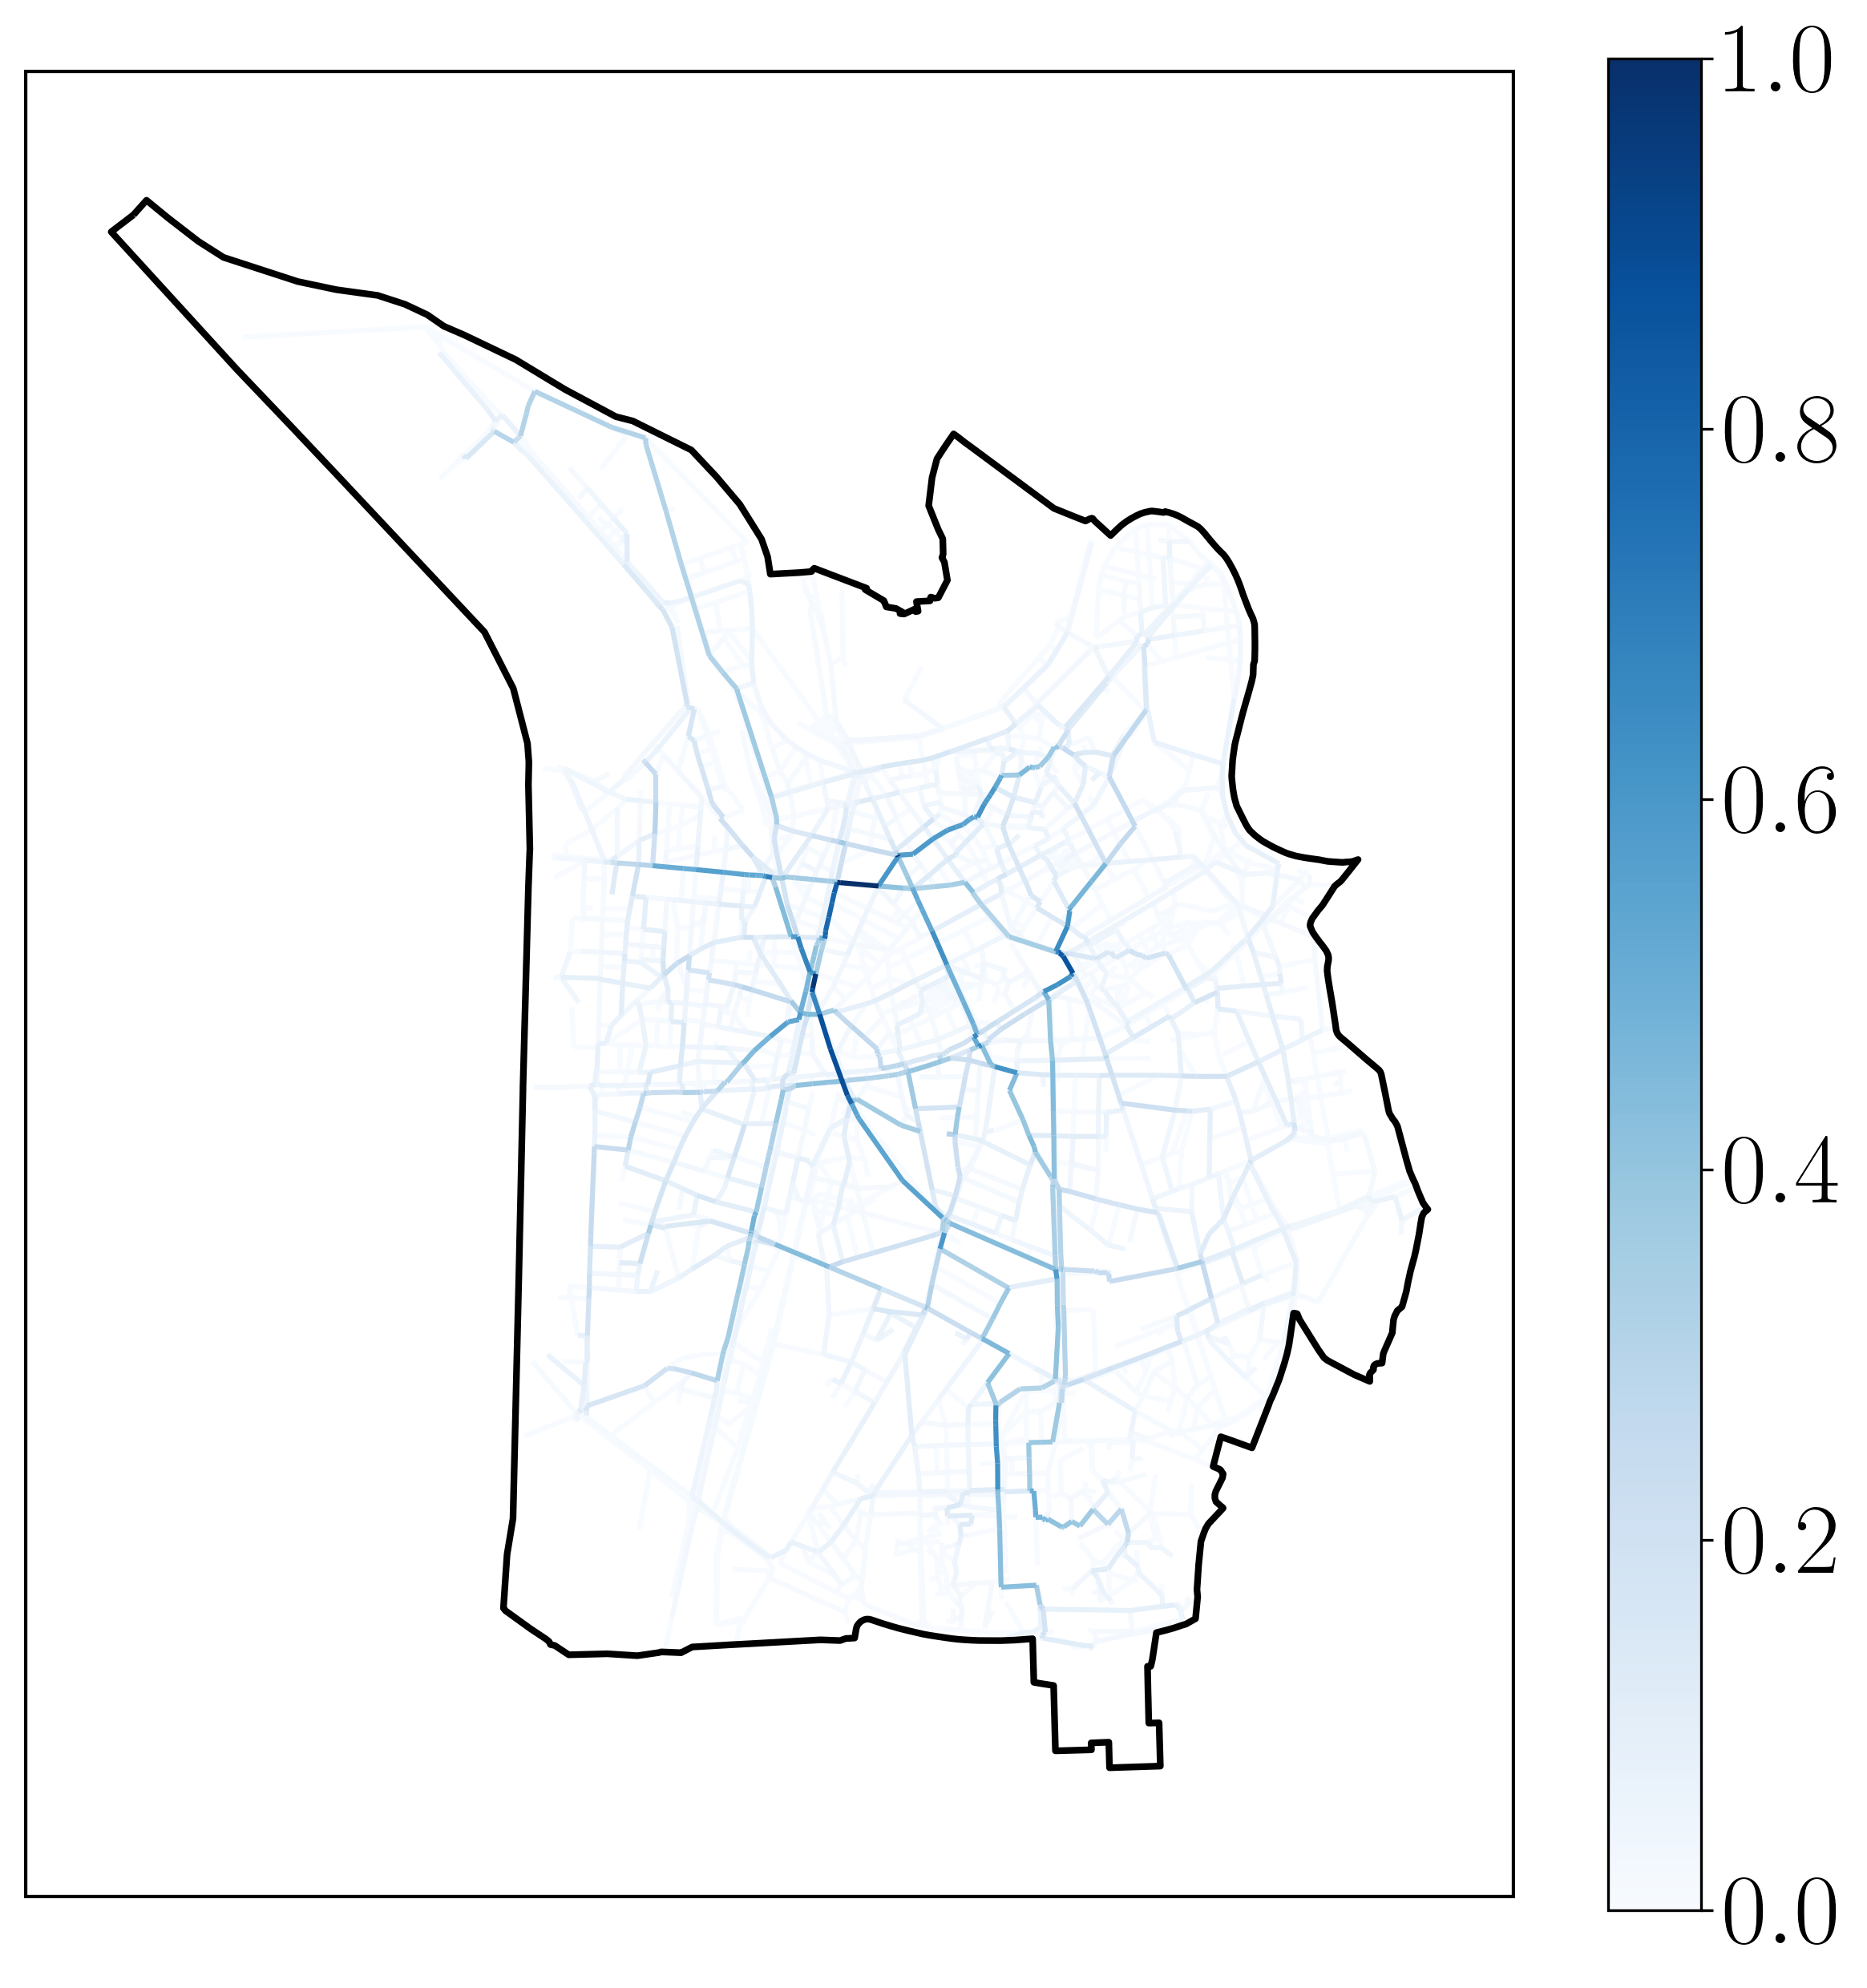
\includegraphics[width=0.23\linewidth]{Images/G_original_flow_3.png}\label{l_2_5_4}}
  % \hspace{0.012\linewidth} % Adjust horizontal space as 
  % \subfloat[MLCC flow]
  % {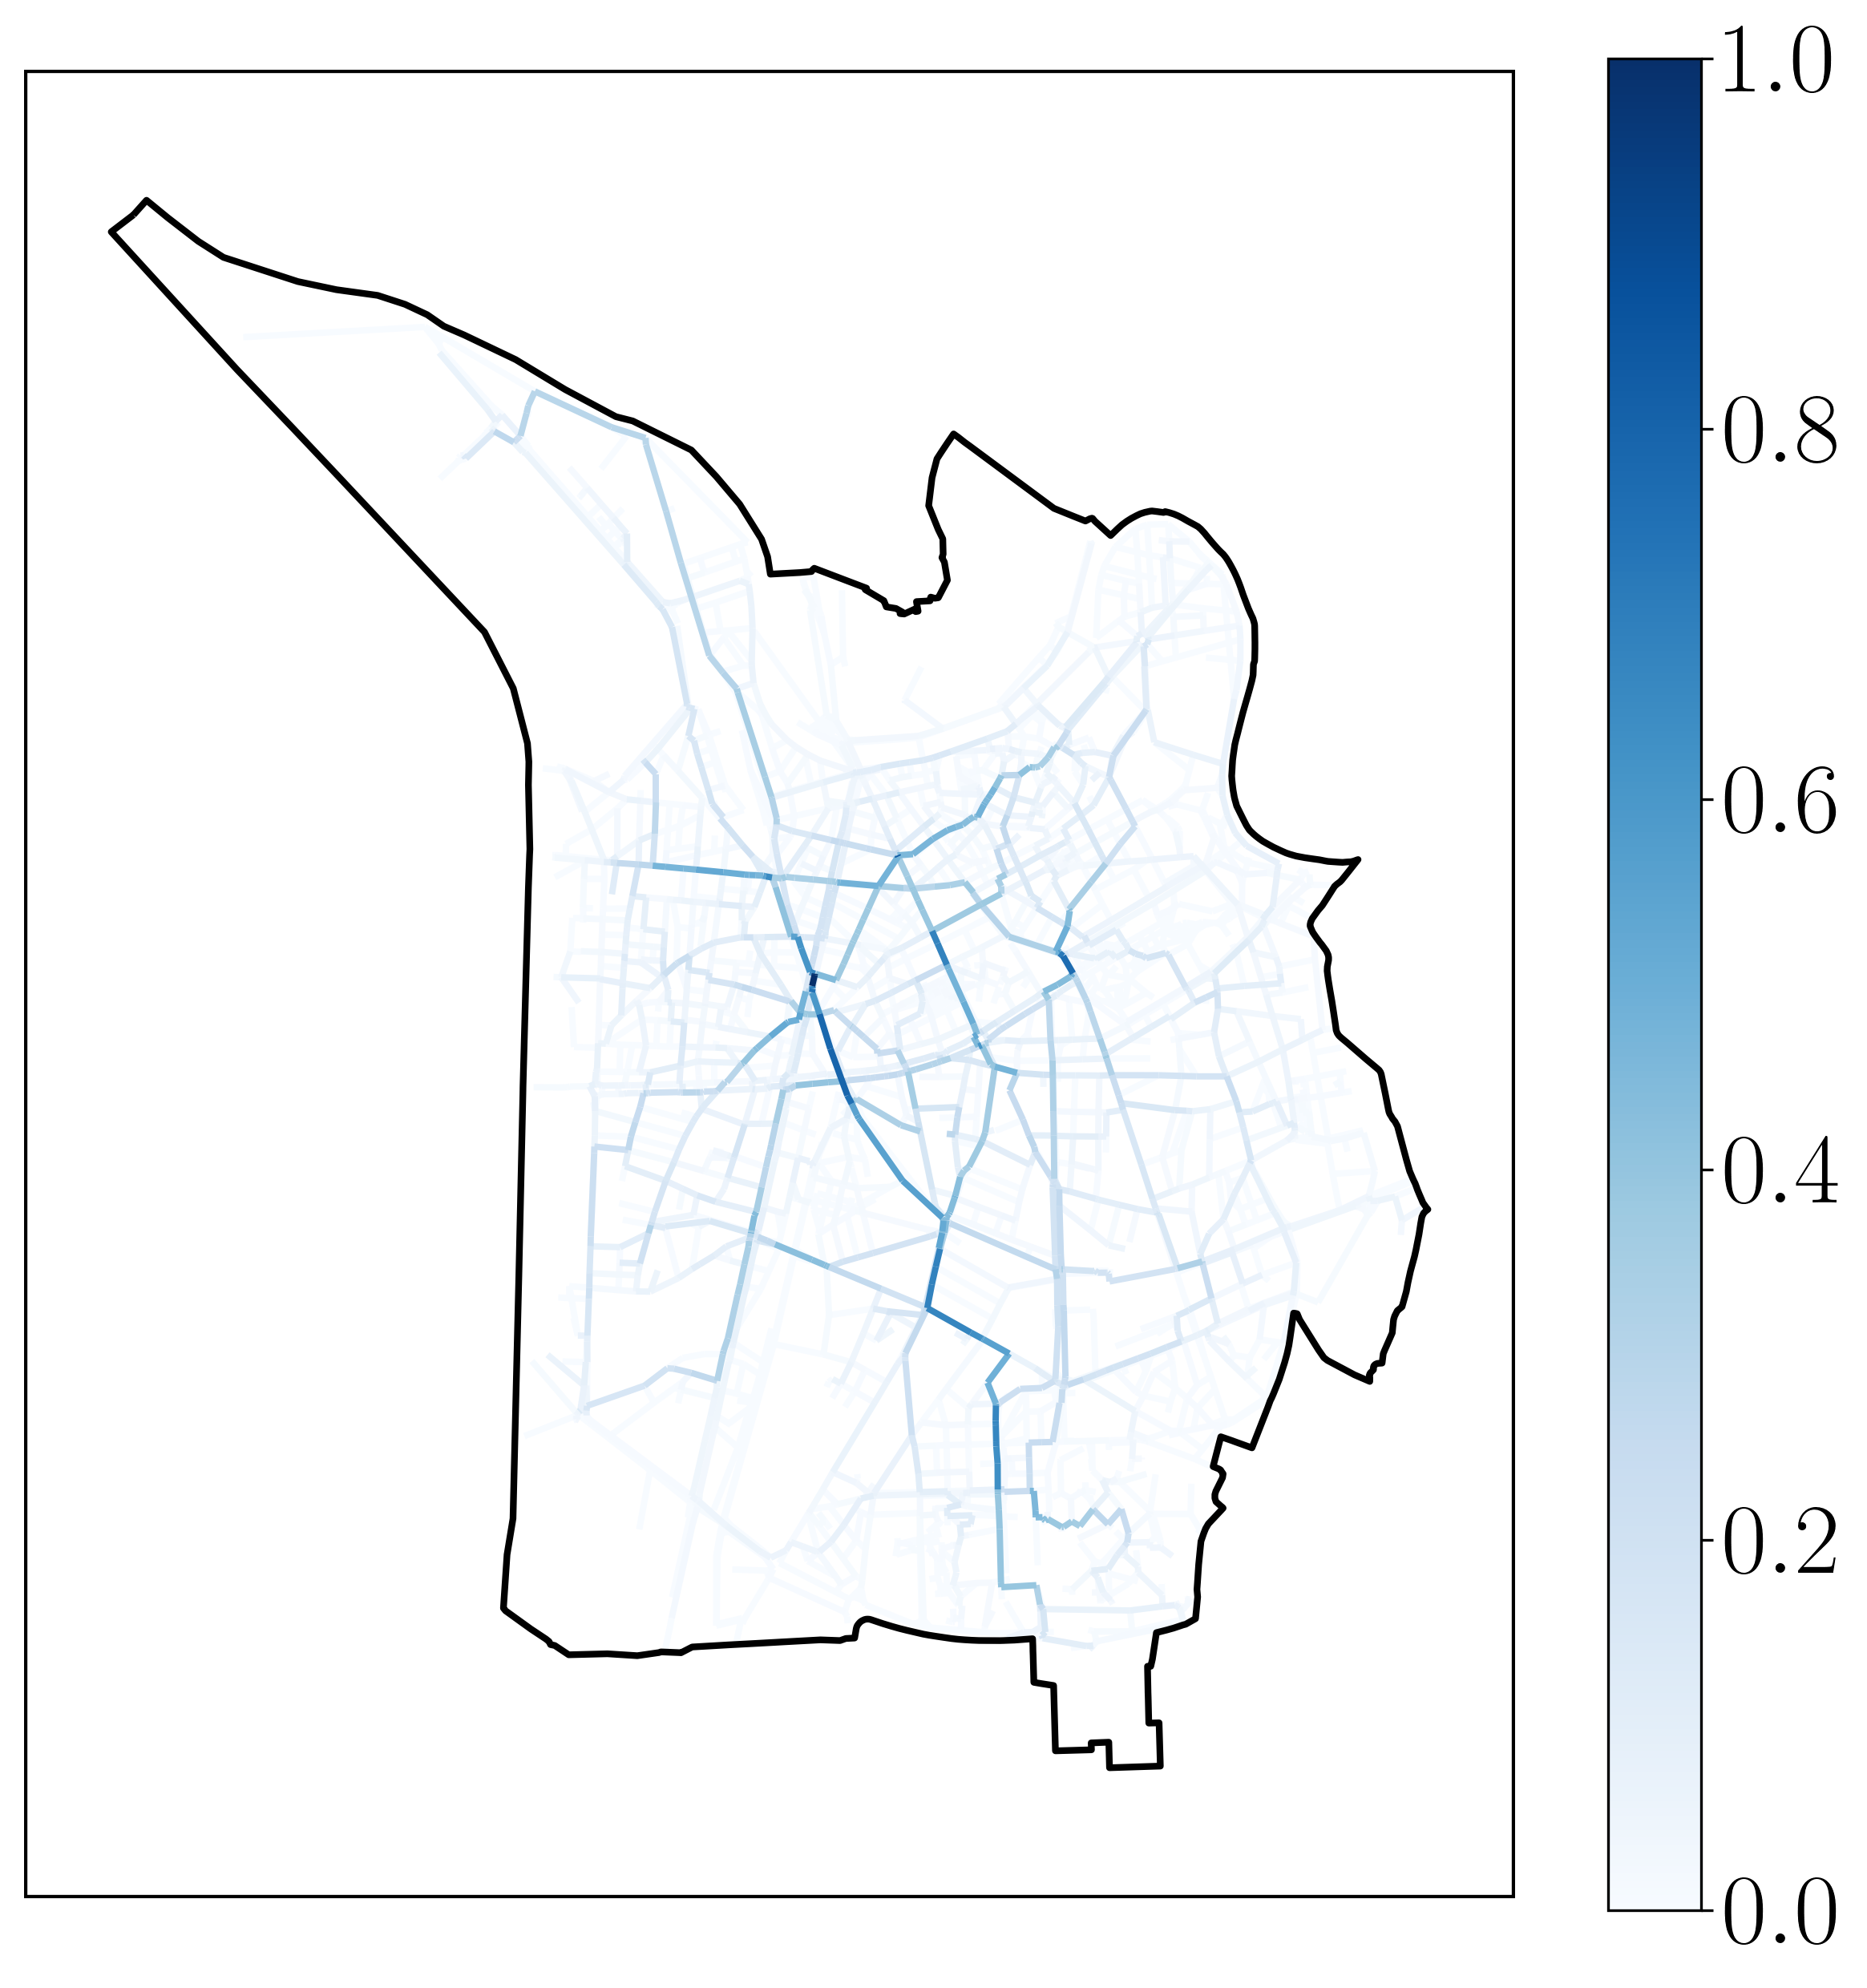
\includegraphics[width=0.23\linewidth]{Images/MLCC_flow_3.png}\label{l_2_5_12}}
  % \hspace{0.012\linewidth}
  % \subfloat[GAB flow]
  % {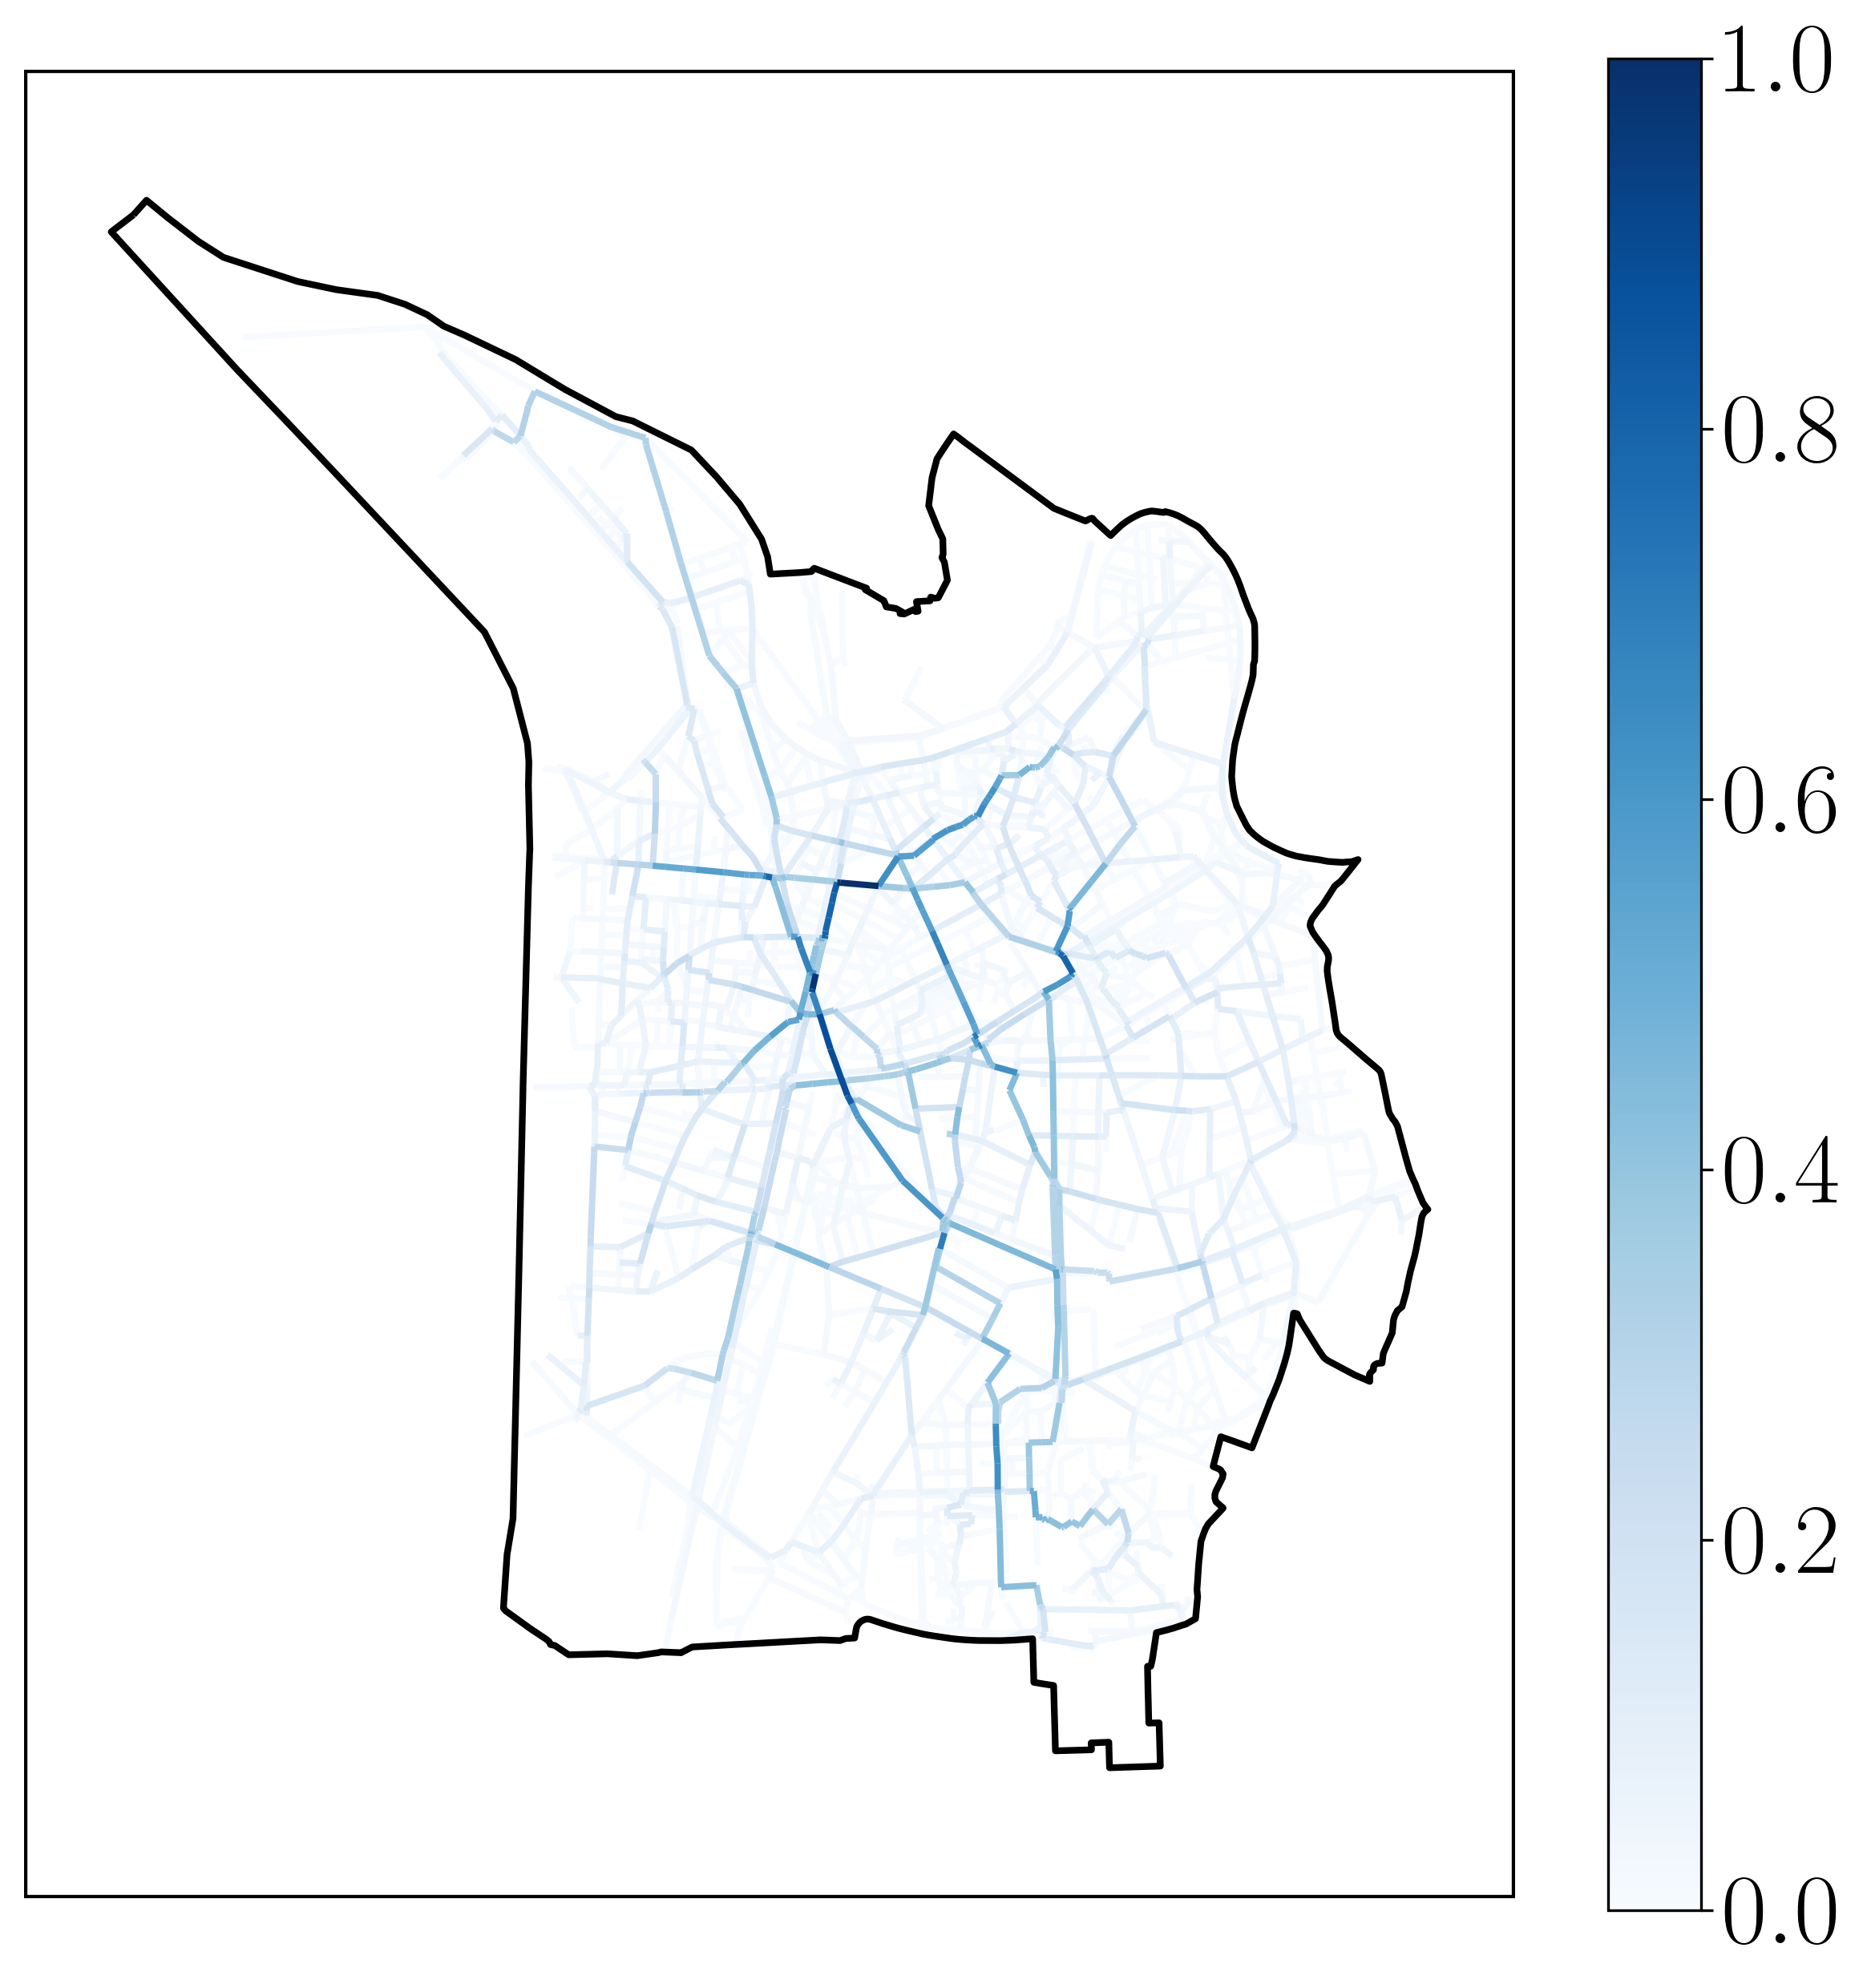
\includegraphics[width=0.23\linewidth]{Images/GAB_flow_3.png}\label{l_2_5_5}}
  % \hspace{0.012\linewidth}
  % \subfloat[GAB-F flow]
  % {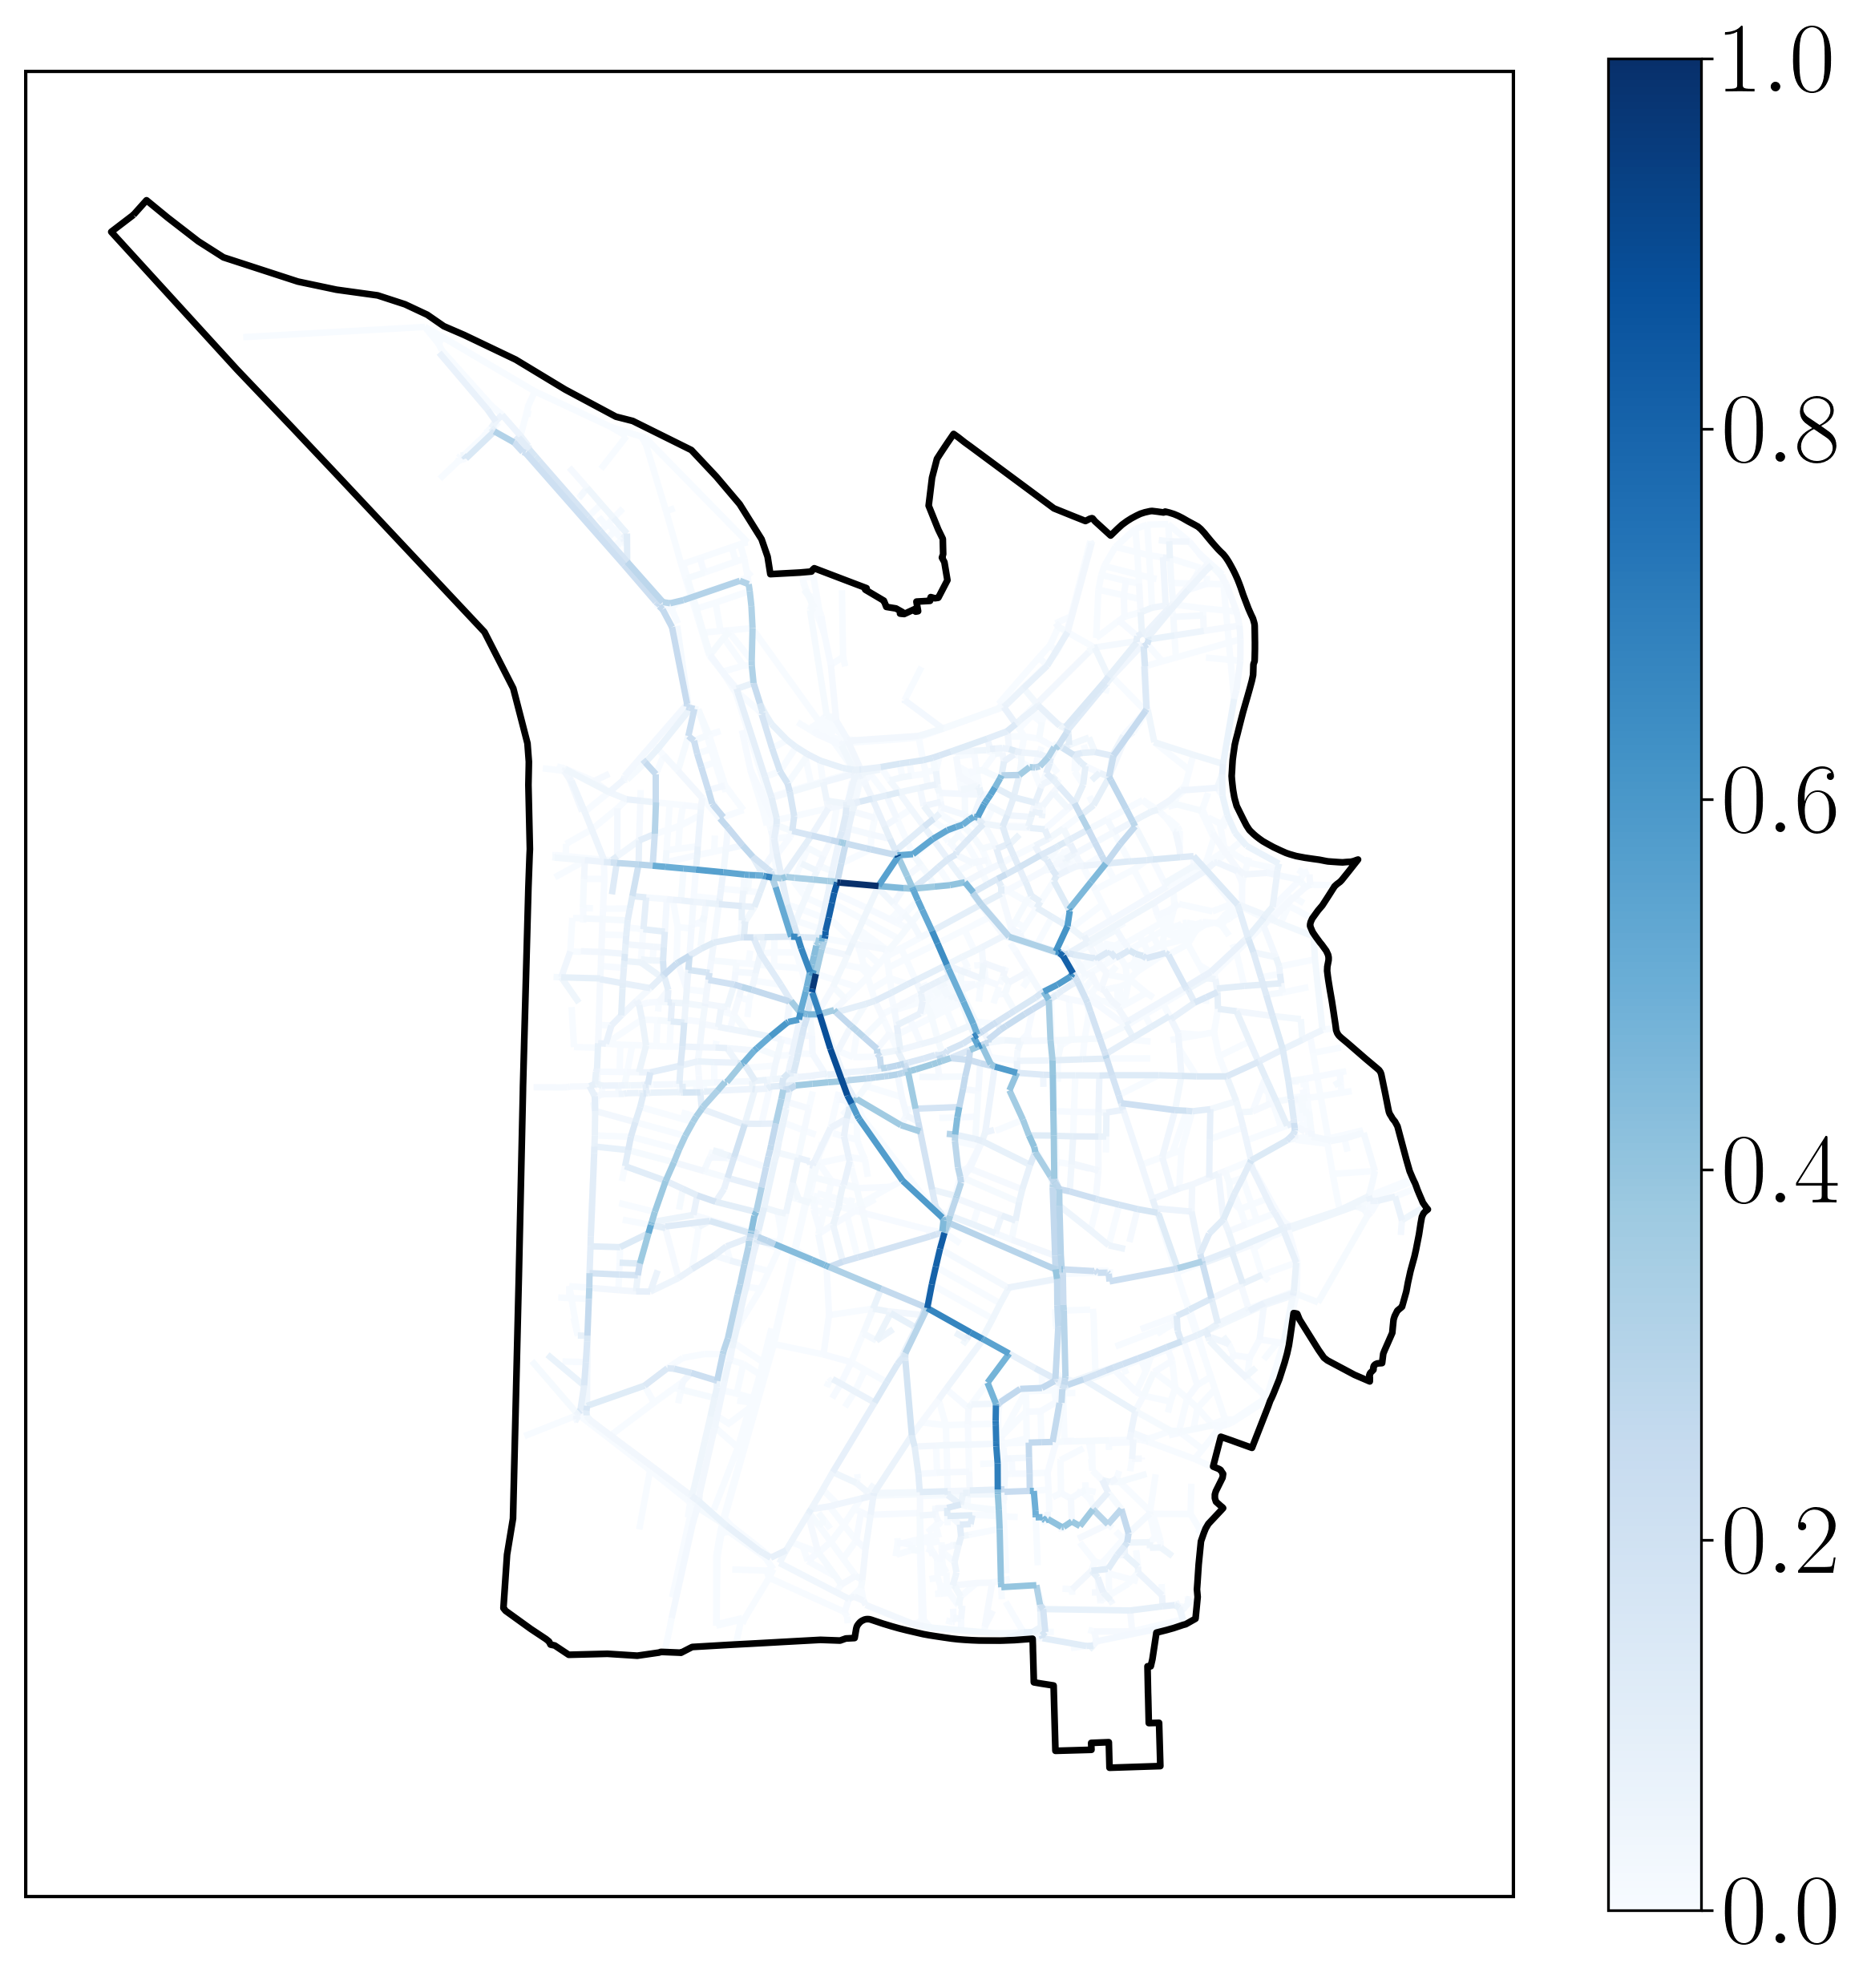
\includegraphics[width=0.23\linewidth]{Images/GAB_F_flow_3.png}\label{l_2_5_6}}\\
  \subfloat[Original insufficiency]{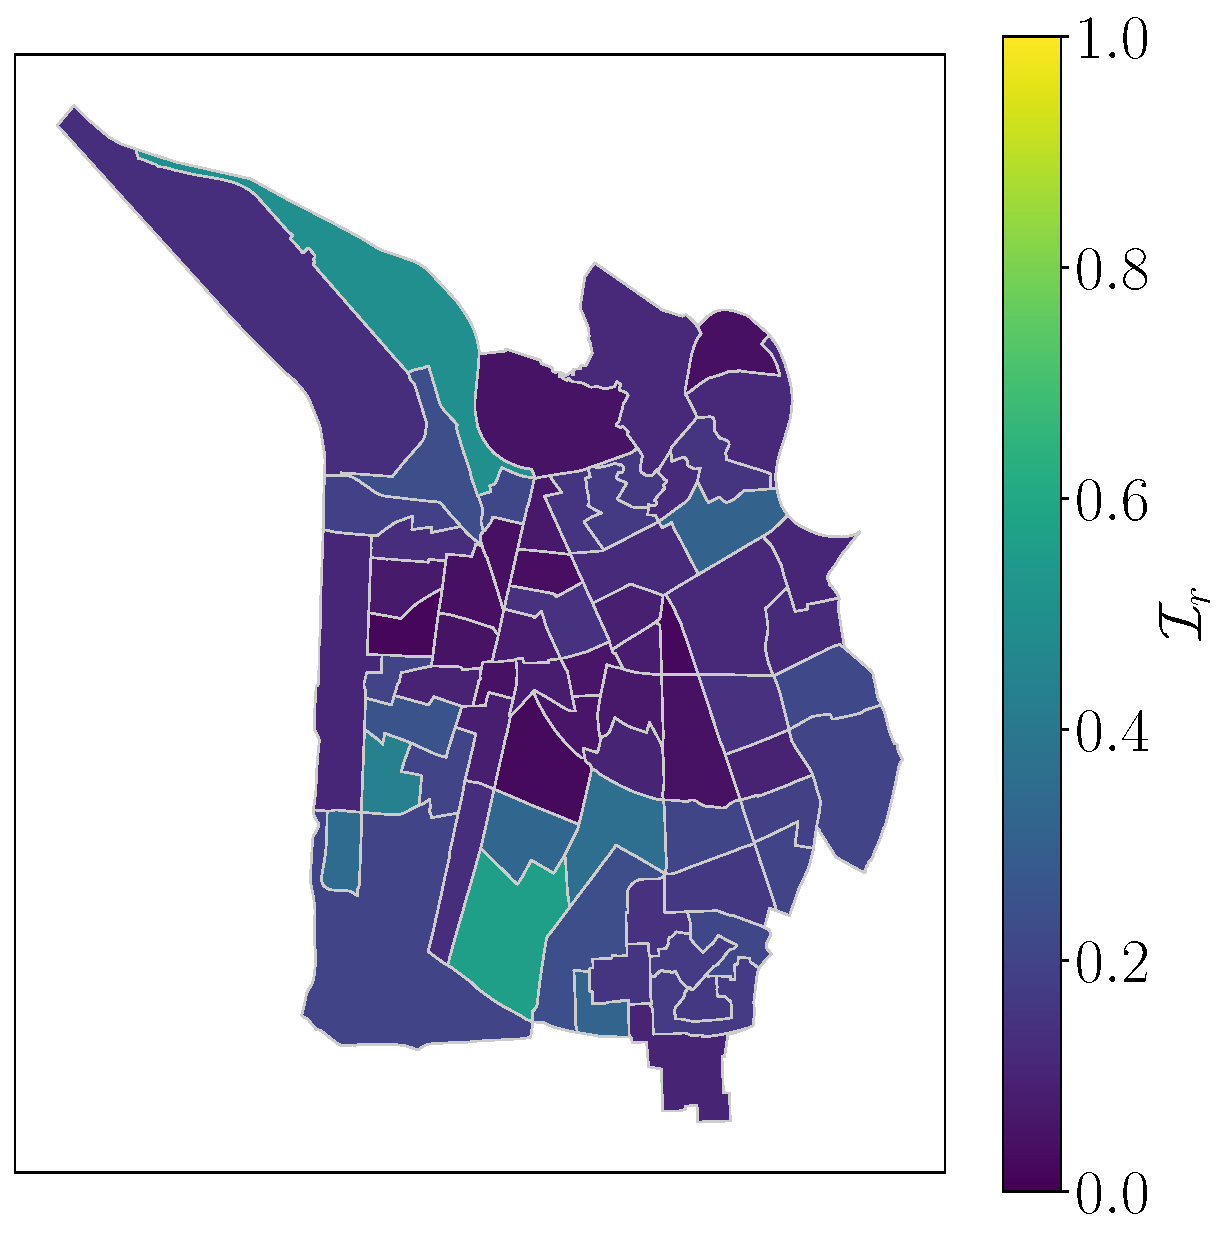
\includegraphics[width=0.24\linewidth]{Images/G_original_regional_3.pdf}\label{l_2_5_7}}
  \hspace{0.004\linewidth} % Adjust horizontal space as 
  \subfloat[MLCC insufficiency]
  {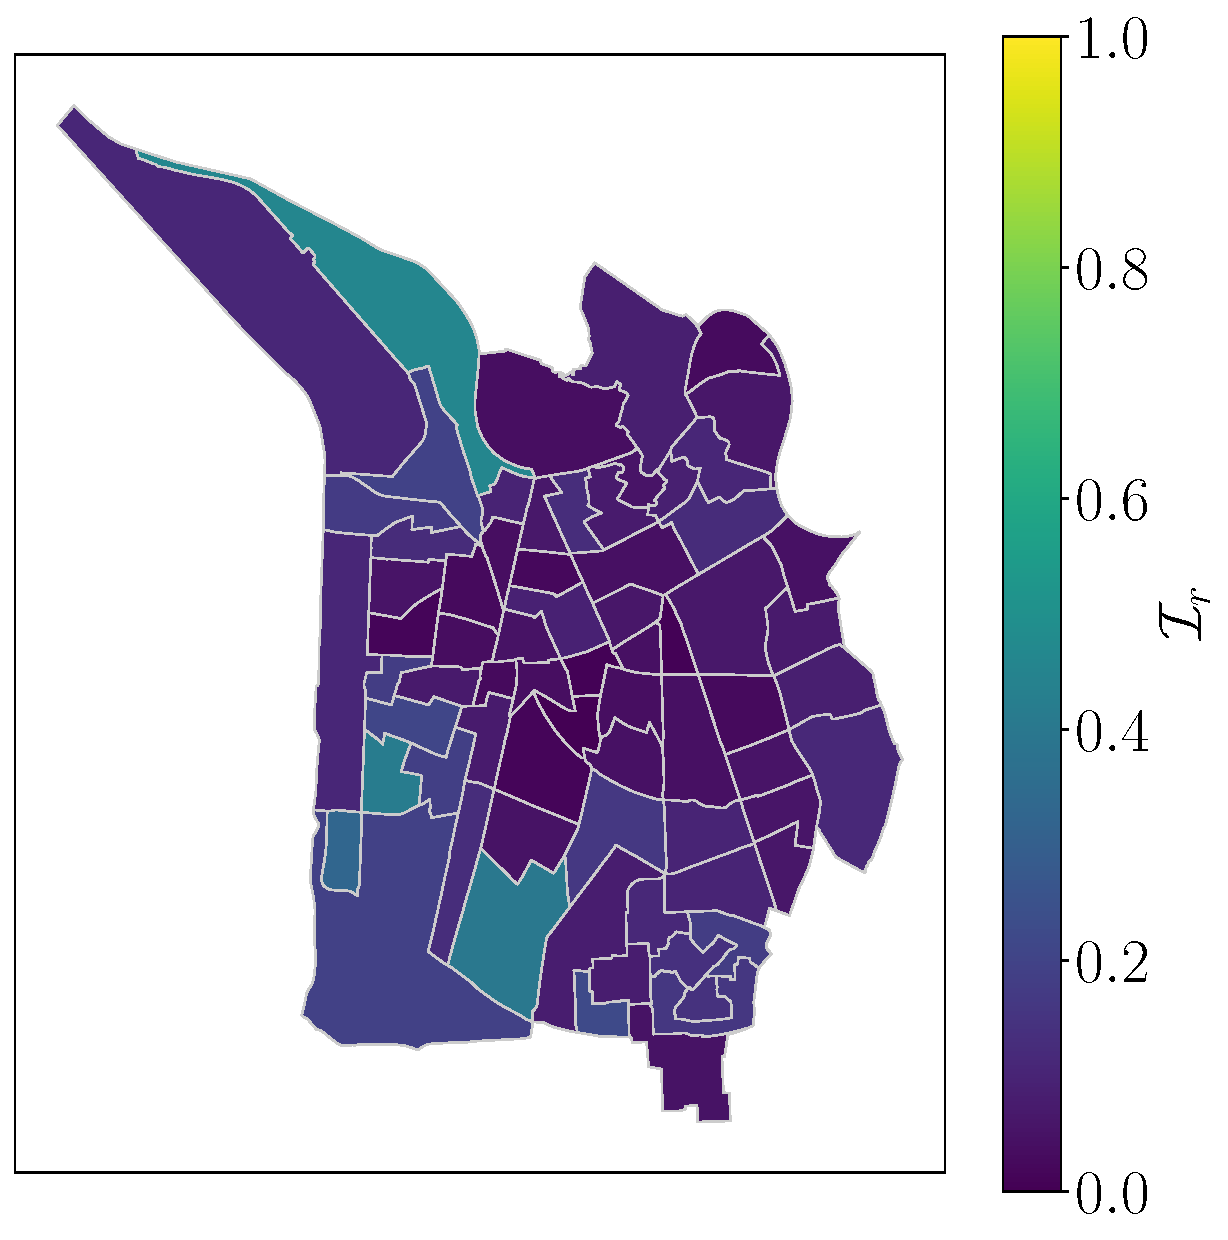
\includegraphics[width=0.24\linewidth]{Images/MLCC_regional_3.pdf}\label{l_2_5_8}}
  \hspace{0.004\linewidth}
  \subfloat[\mbox{GA-U} insufficiency]
  {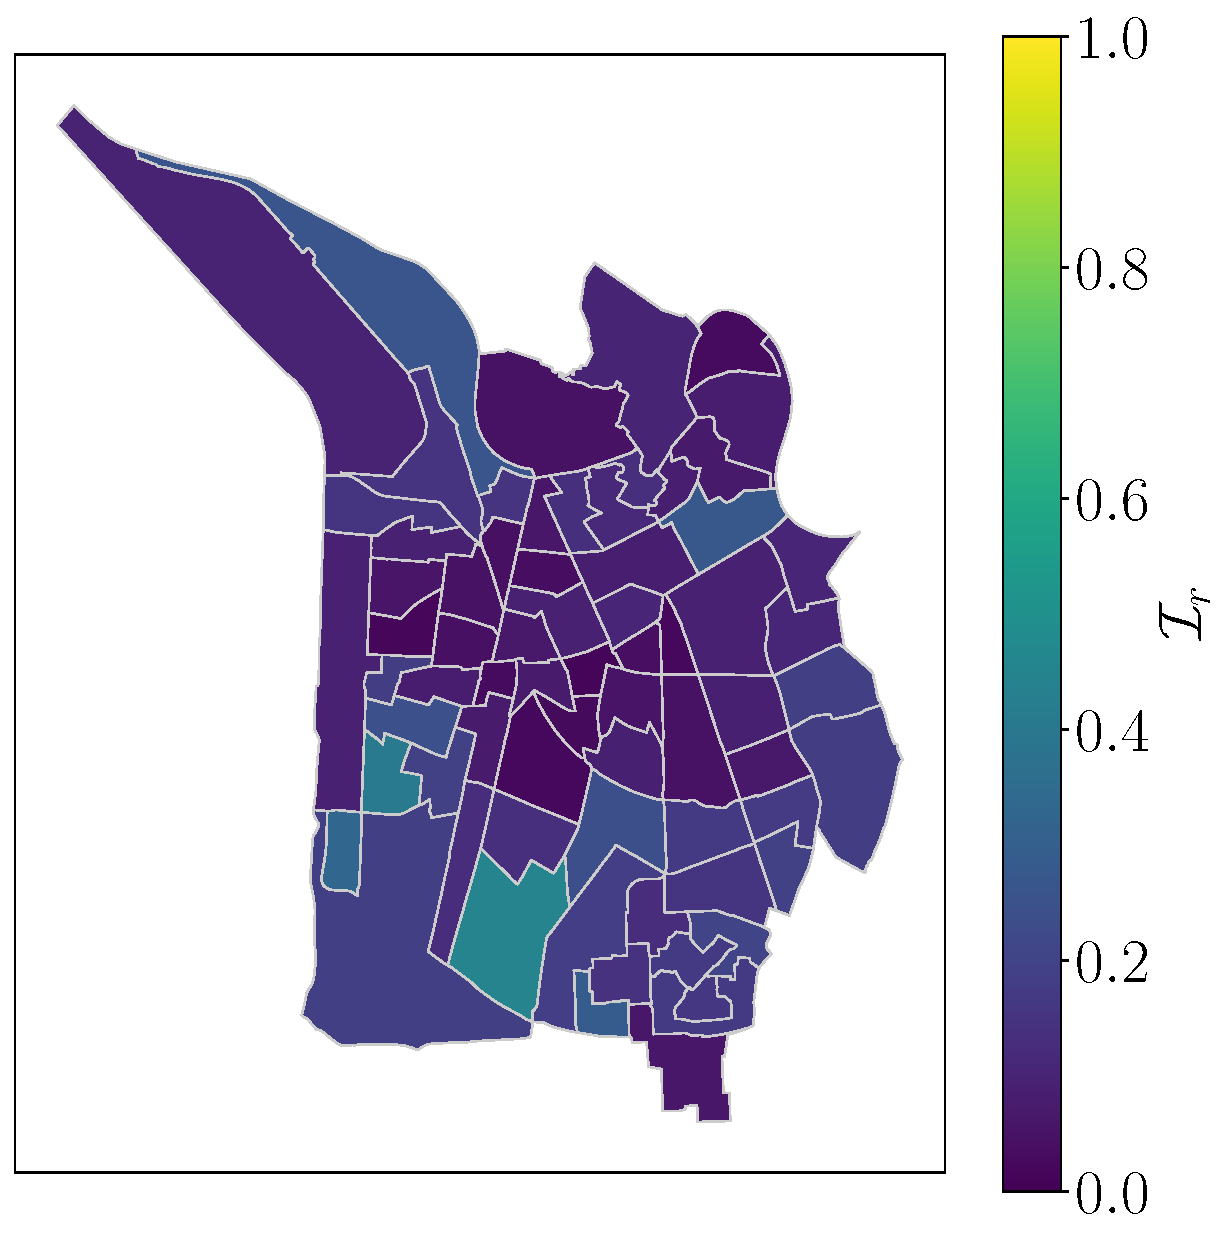
\includegraphics[width=0.24\linewidth]{Images/GAB_regional_3.pdf}\label{l_2_5_9}}
  \hspace{0.004\linewidth}
  \subfloat[\mbox{GA-S} insufficiency]
  {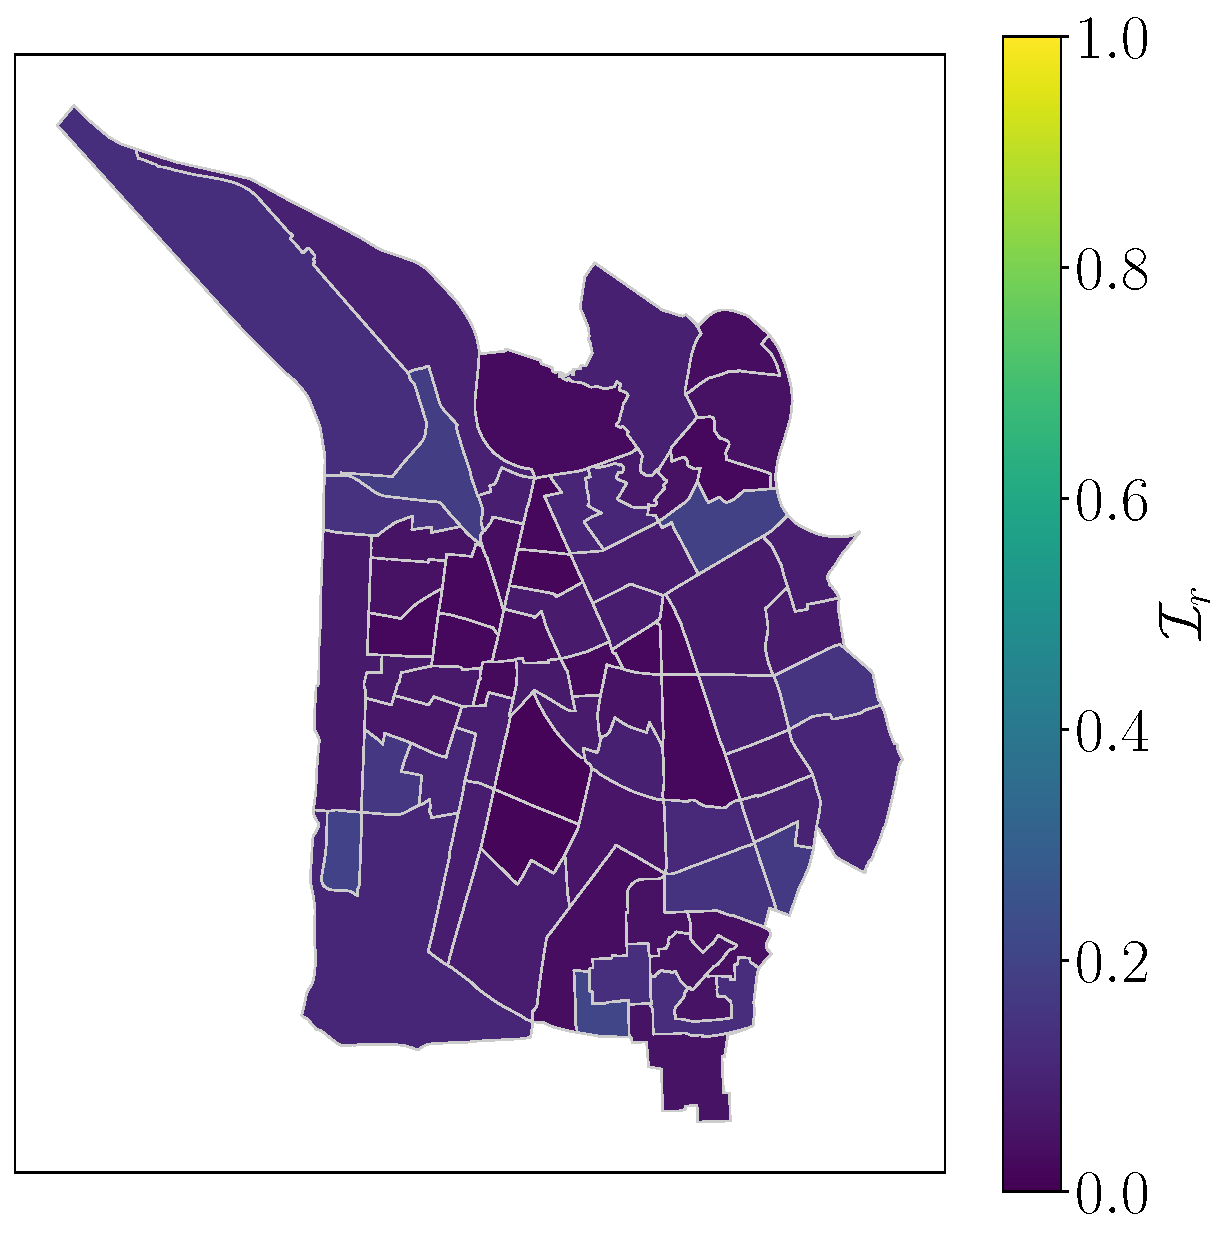
\includegraphics[width=0.24\linewidth]{Images/GAB_F_regional_3.pdf}\label{l_2_5_10}}
   
  
  \caption{\footnotesize The top section displays the DoS configuration, while the bottom illustrates regional safety insufficiency. The optimization algorithms are applied with $\lambda=40\%$ and a budget of $B^{\ast}_{\lambda}\approx0.056 \cdot B_{\max}$.}
  \label{grenoble_lambda_2_5}
\end{figure*}

\begin{figure}[h!]
\vspace{0.2cm}
  \centering
  \captionsetup[subfigure]{font={footnotesize}, labelfont={footnotesize, bf}, textfont={footnotesize, rm}}

  \subfloat[Original]{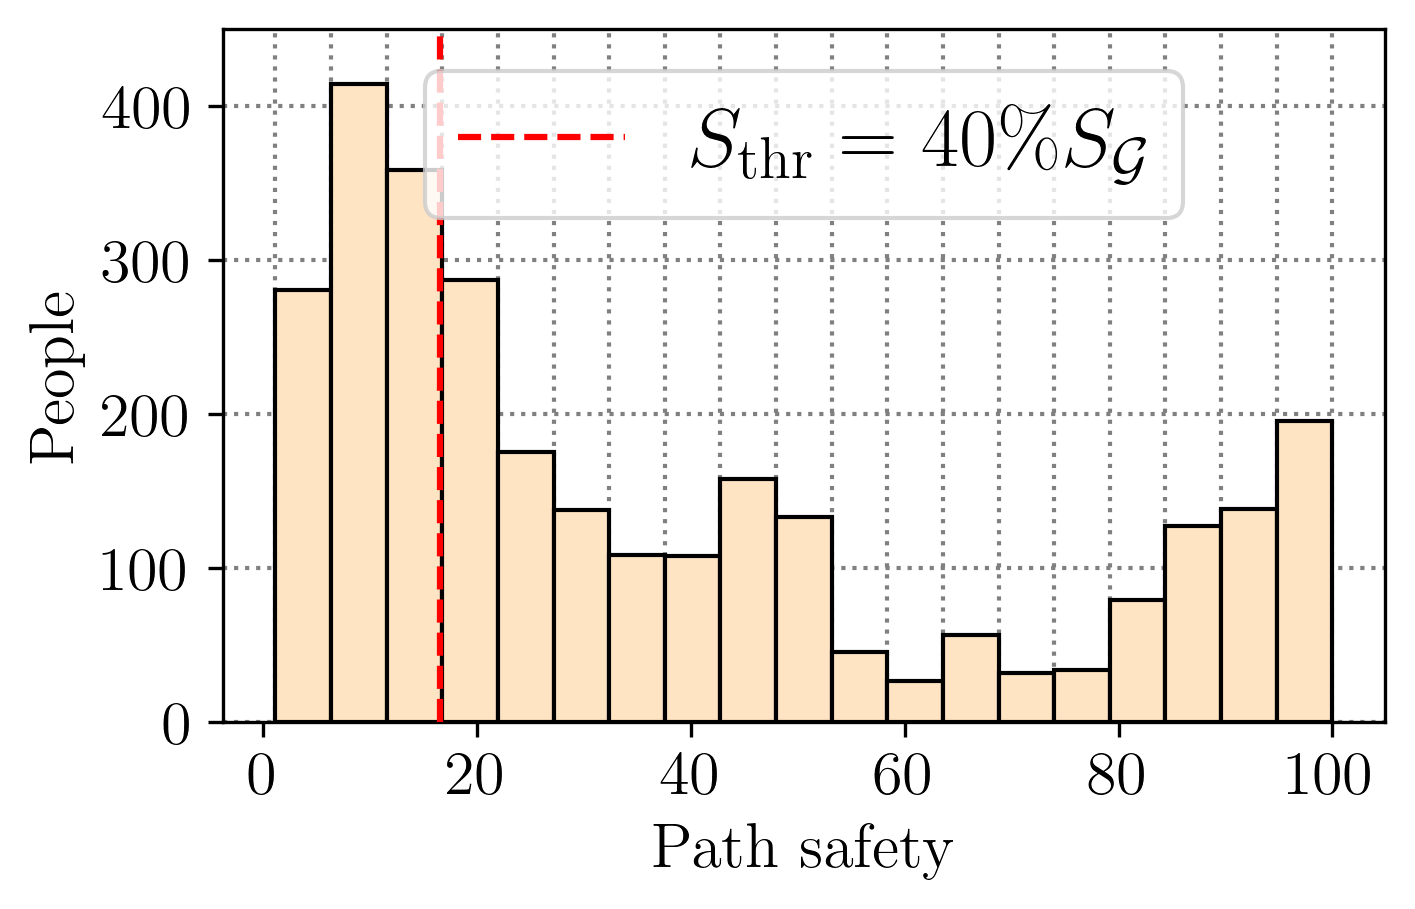
\includegraphics[width=0.48\linewidth]{Images/histogram_3_0.png}\label{hist_1}}
  \hspace{0.001\linewidth}
  % \hspace{0.001\linewidth} % Adjust horizontal space as needed
  \subfloat[MLCC]
  {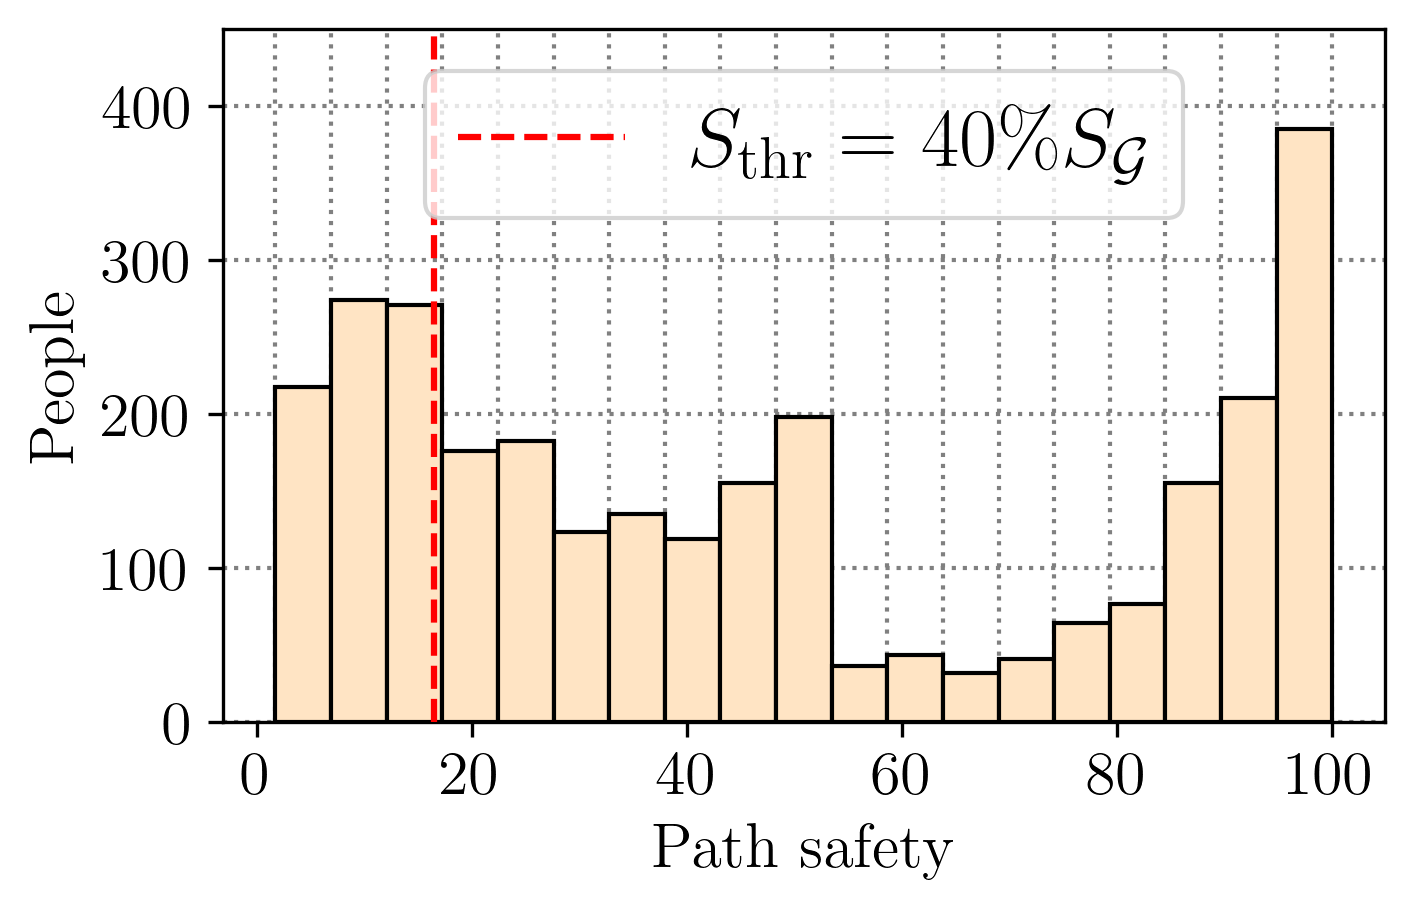
\includegraphics[width=0.48\linewidth]{Images/histogram_3_1.png}\label{hist_2}} \\
  \vspace{0.001\linewidth} % Adjust horizontal space as needed
  \subfloat[\mbox{GA-U}]{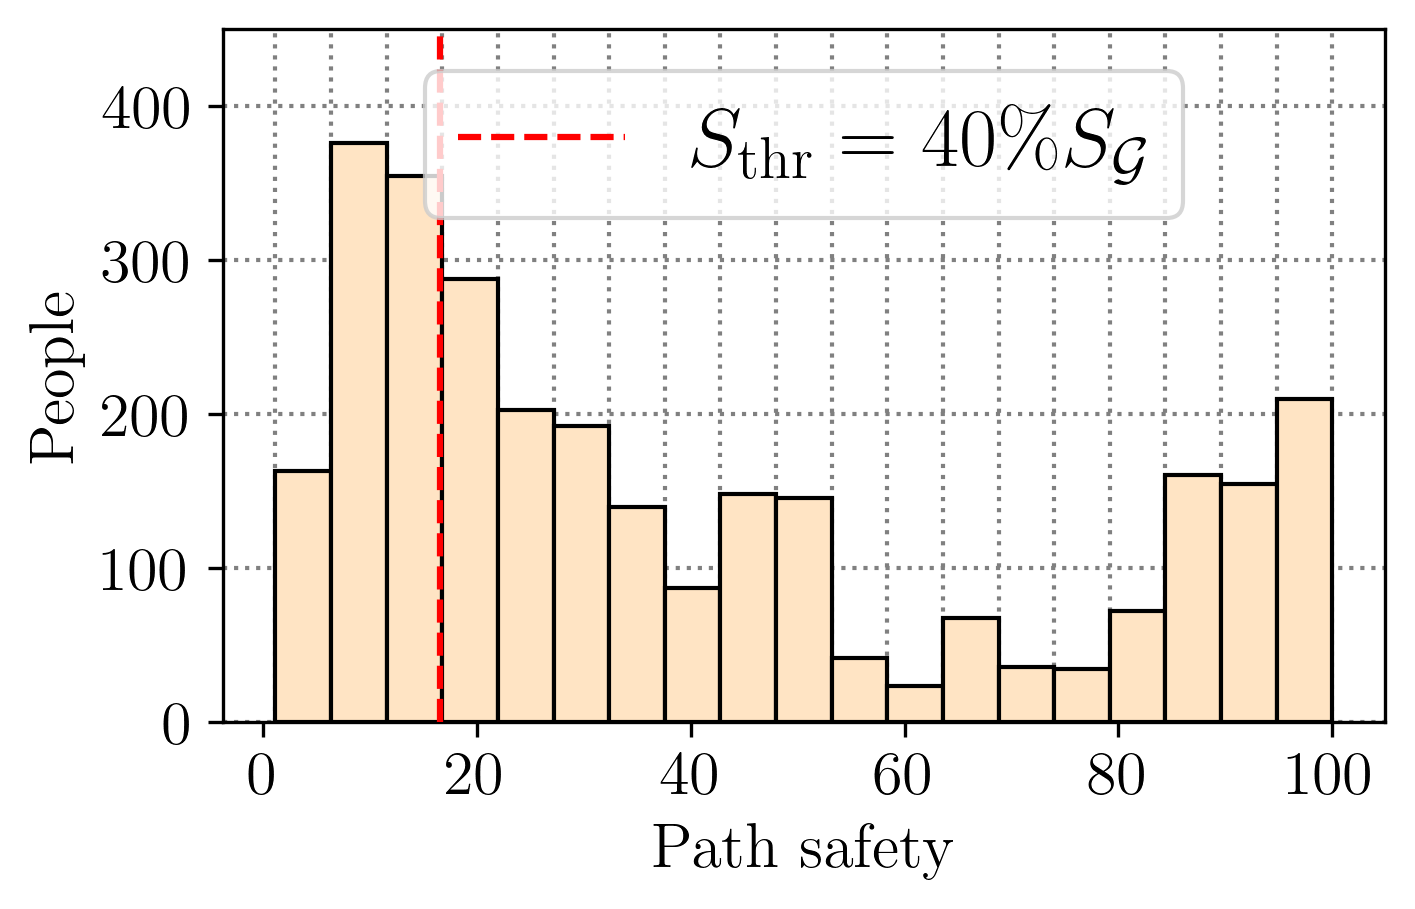
\includegraphics[width=0.48\linewidth]{Images/histogram_3_2.png}\label{hist_3}}
  \hspace{0.001\linewidth} % Adjust vertical space as needed
  \subfloat[\mbox{GA-S}]{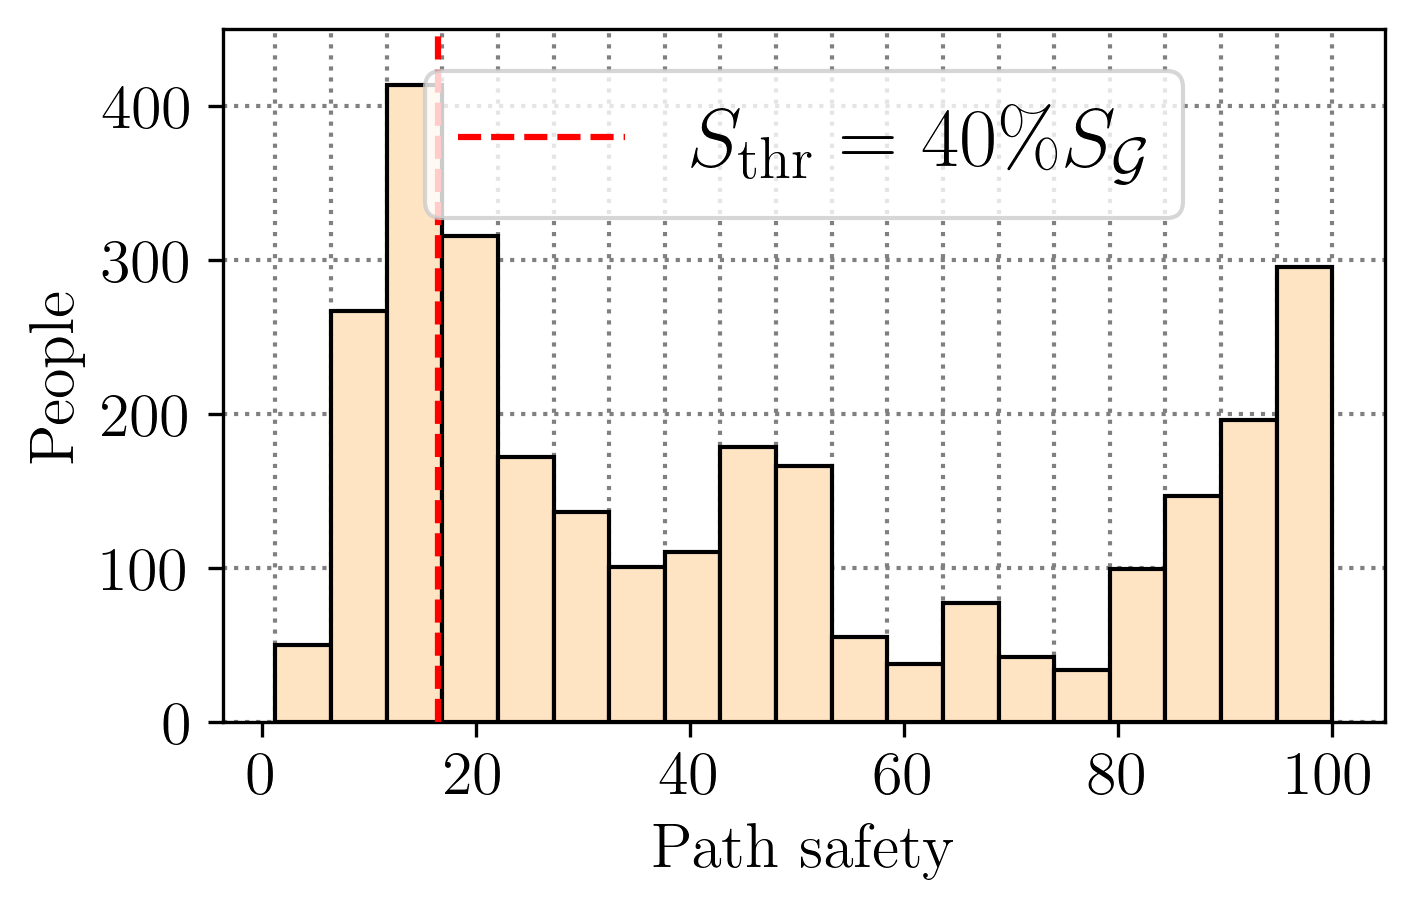
\includegraphics[width=0.48\linewidth]{Images/histogram_3_3.png}\label{hist_4}}
  \caption{\footnotesize Path safety versus the number of individuals above and below the threshold $\lambda=40\%$ and a budget of $B^{\ast}_{\lambda}\approx0.056 \cdot B_{\max}$.}
  \label{histograms_plots}
\end{figure}
\begin{equation}
B_k = B_{\min} + \left(\frac{B_{\max}}{2} - B_{\min}\right) \cdot \frac{\log(k)}{\log(10)}, \quad k \in \{1, \dots, 10\},
\end{equation}
where $B_{\min} = \frac{B_{\max}}{100}$ constrains the budget range to $\left[ \frac{B_{\max}}{100}, \frac{B_{\max}}{2} \right]$. This ensures denser sampling near smaller budgets, capturing significant marginal improvements while remaining realistic for practical applications. The resulting budget values are approximately
\begin{equation}
    \begin{array}{r}
           B_{k} \approx [0.01,  0.015,  0.023,  0.036,  0.056,  \\ 
         0.087,  0.135,  0.209,  0.323,  0.5] \cdot B_{\max}.
    \end{array}
\end{equation}

To identify the budget that significantly improves safety while affecting the safety inssuficiency, we fix the safety threshold parameter $\lambda~\in~\left \{  10\%,20\%,30\%,40\%,50\% \right \}$ and solve Problem 2 for each $B_k$. The corresponding solution is denoted as $\mathbf{w}^{\star} (B_k, \lambda)$, and we compute the marginal improvements as follows:
    \begin{equation}
    \Delta \mathbf{w}^{\star} (B_k, \lambda) = \mathbf{w}^{\star}(B_{k-1}, \lambda) - \mathbf{w}^{\star}(B_{k}, \lambda).
    \end{equation}
The budget $B^{\star}_{\lambda}$ is identified as
\begin{equation}
\label{marginal}
B^{\star}_{\lambda} = \arg\max_{B_k} \left( \frac{\Delta \mathbf{w}^{\star} (B_k, \lambda)}{B_k - B_{k-1}} 
\right),    
\end{equation}
where larger marginal improvements relative to budget increases are prioritized. However, higher budgets do not always yield greater marginal gains, as the impact depends on the specific upgrades made possible by the additional funds, often leading to diminishing returns at higher budget levels. Then, Problems~1 and 2 are solved for $B^{\ast}_{\lambda}$ for each $\lambda$ using the MLCC, \mbox{GA-U}, and \mbox{GA-S} algorithms in our study case.






\subsection{Grenoble Case Study}

Our case study focuses on the Grenoble cycling network. The results of solving \eqref{marginal} are presented in Fig.~\ref{marginal_plot}, which illustrates the budget required for each threshold $\lambda$. Specifically, for $\lambda \in \left \{10\%,20\%,30\%,40\% \right \}$, the maximum marginal improvement relative to the budget increase occurs at $B_{\lambda}^{\ast} \approx~0.056~\cdot B_{\max}$. When $\lambda~=~50\%$, this value increases to $B_{\lambda}^{\ast}~\approx~0.087~\cdot~B_{\max}$. This suggests that at higher safety thresholds, optimization may require additional investments before reaching the point of maximum marginal improvement, possibly due to stricter budget allocation constraints. Consequently, the analysis is conducted using these budget levels. To illustrate this, Fig.~\ref{grenoble_lambda_2_5} presents the original DoS distribution and regional safety insufficiency, together with the corresponding results after applying the optimization MLCC, \mbox{GA-U} and \mbox{GA-S} for $\lambda=40\%$. In Fig.~\ref{grenoble_lambda_2_5}(\textbf{b}), MLCC allocates the entire budget to connect previously disconnected components with high DoS scores using the safest available paths. Conversely, \mbox{GA-U}, shown in Fig.~\ref{grenoble_lambda_2_5}(\textbf{c}), distributes the budget more evenly across the network. However, \mbox{GA-S} reduces the best regional safety insufficiency, as seen in Fig.~\ref{grenoble_lambda_2_5}(\textbf{e}$-$\textbf{h}).  Fig.~\ref{histograms_plots} presents the relationship between path safety scores and the number of cyclists in each case. Although MLCC achieves the highest number of individuals with the safest paths, \mbox{GA-S} exceeds it by ensuring that more individuals exceed the threshold. Fig.~\ref{above_below} displays the percentage of individuals above and below the threshold for each $\lambda$. As $\lambda$ increases, the proportion of individuals below the threshold increases. However, in all cases, \mbox{\mbox{GA-S}} consistently reduces the number of individuals below the threshold more effectively than the other methods.

\begin{figure}[t]
\vspace{0.2cm}
  \centering
  \captionsetup[subfigure]{font={footnotesize}, labelfont={footnotesize, bf}, textfont={footnotesize, rm}}

  \subfloat[$\lambda=10\%$]{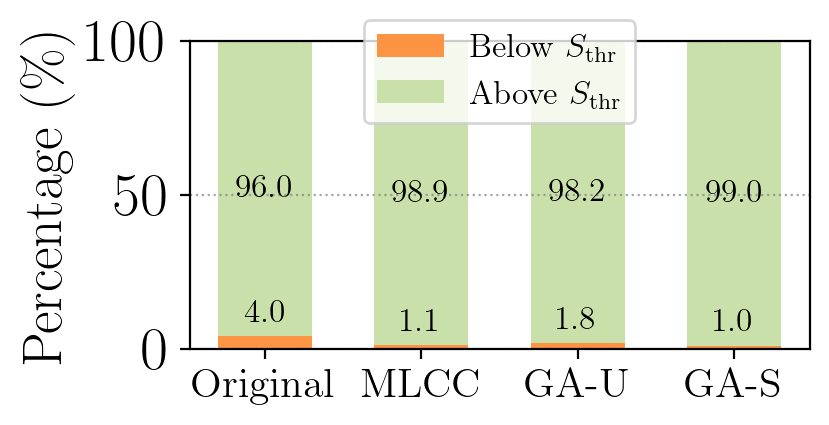
\includegraphics[width=1\linewidth]{Images/threshold_distribution_0.png}\label{above_below_1}}\\
  % \hspace{0.001\linewidth} % Adjust horizontal space as needed
  \subfloat[$\lambda=20\%$]{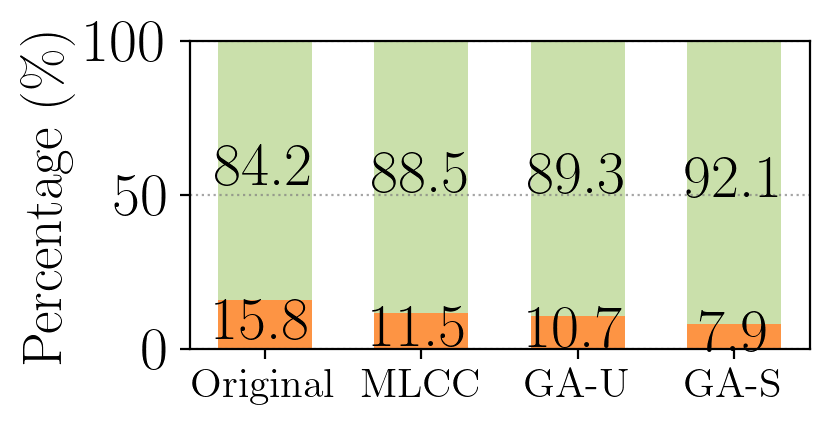
\includegraphics[width=0.48\linewidth]{Images/threshold_distribution_1.png}\label{above_below_2}}
  \hspace{0.001\linewidth}
  \subfloat[$\lambda=30\%$]{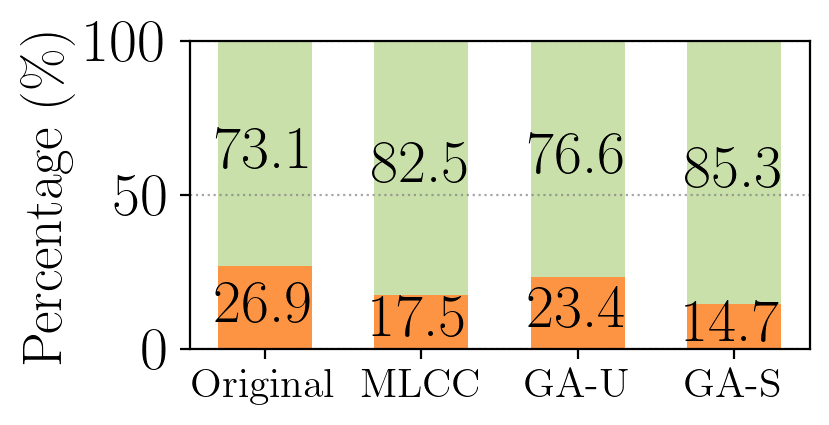
\includegraphics[width=0.48\linewidth]{Images/threshold_distribution_2.png}\label{above_below_3}}\\
  \vspace{0.001\linewidth} % Adjust horizontal space as needed
  \subfloat[$\lambda=40\%$]{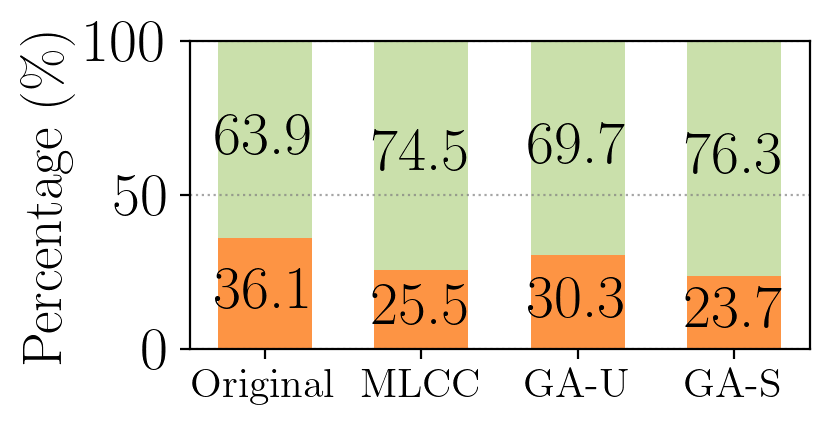
\includegraphics[width=0.48\linewidth]{Images/threshold_distribution_3.png}\label{above_below_4}}
  \hspace{0.001\linewidth}
  \subfloat[$\lambda=50\%$]
  {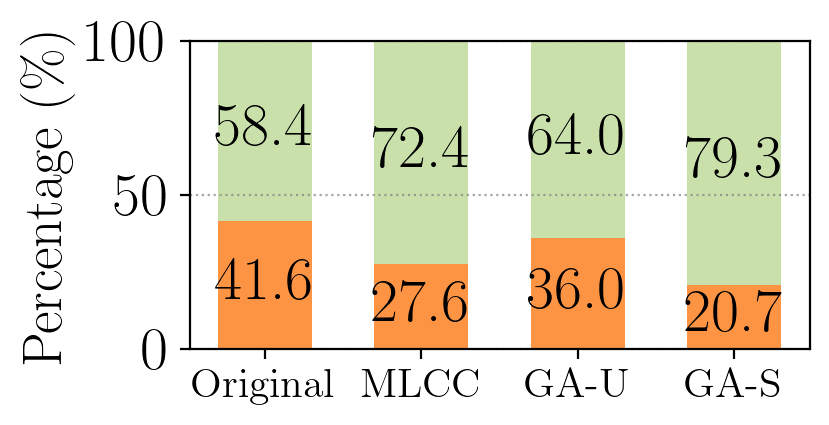
\includegraphics[width=0.48\linewidth]{Images/threshold_distribution_4.png}\label{above_below_5}}
  \caption{\footnotesize Percentage of people above and below the threshold for different $\lambda$ and solutions.}
  \label{above_below}
\end{figure}

\begin{figure}[h!]
\vspace{0.2cm}
\centering
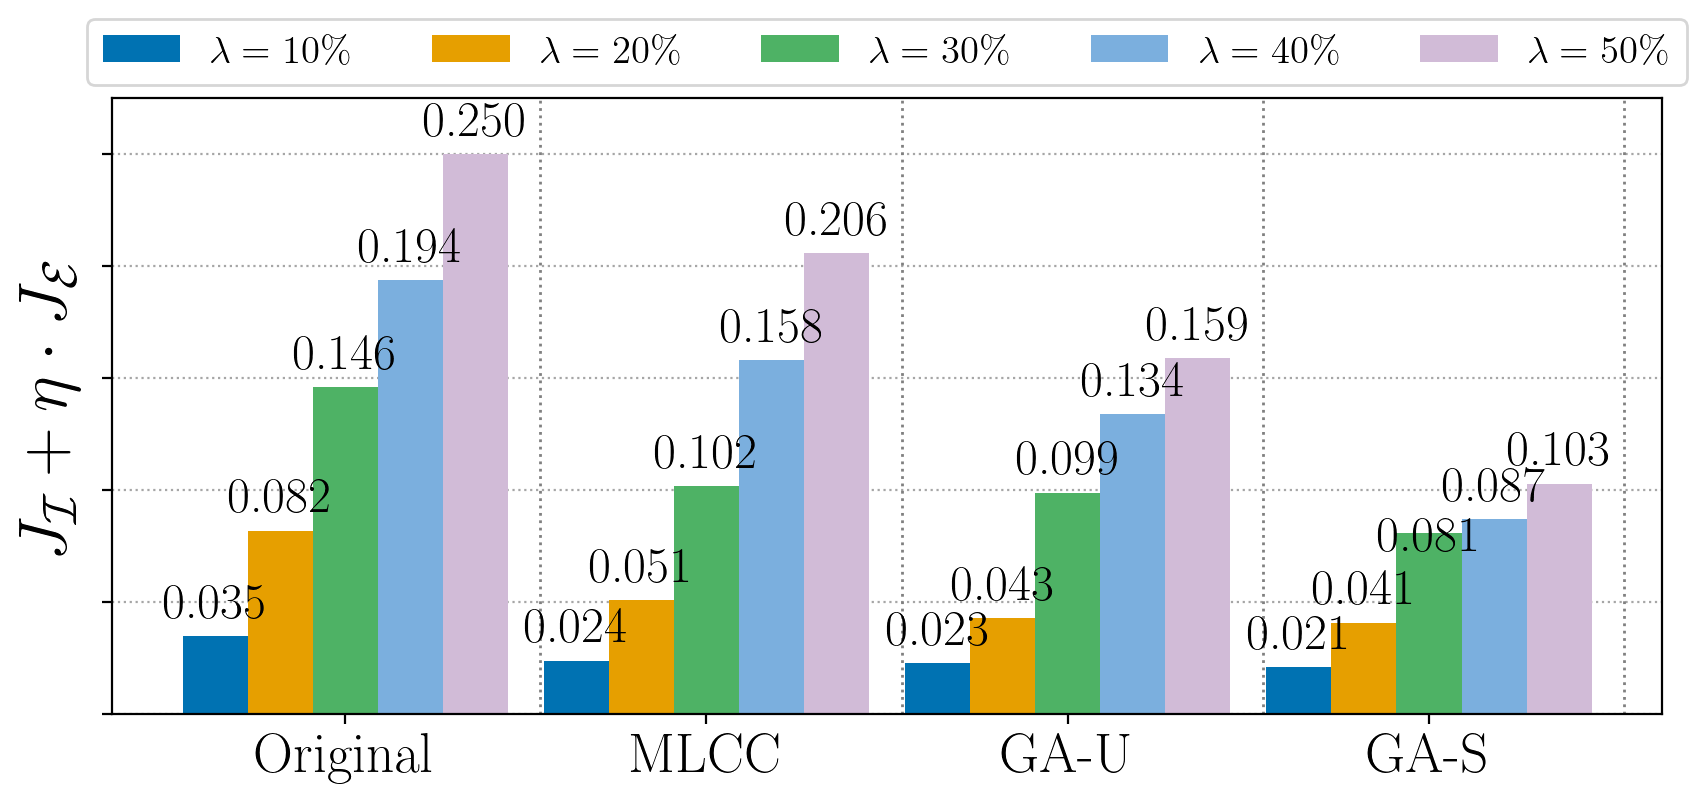
\includegraphics[width=\columnwidth]{Images/unfairness_comparison.png}
\caption{\footnotesize Safety insufficiency comparison of upper level $\mathbb{U}_{\text{thr}}$ of Problem~2, $\eta=0.5$, and the color legend indicates the $\lambda$ threshold.}
\label{unfairness_result}
\end{figure}

\begin{figure}[h!]
\centering
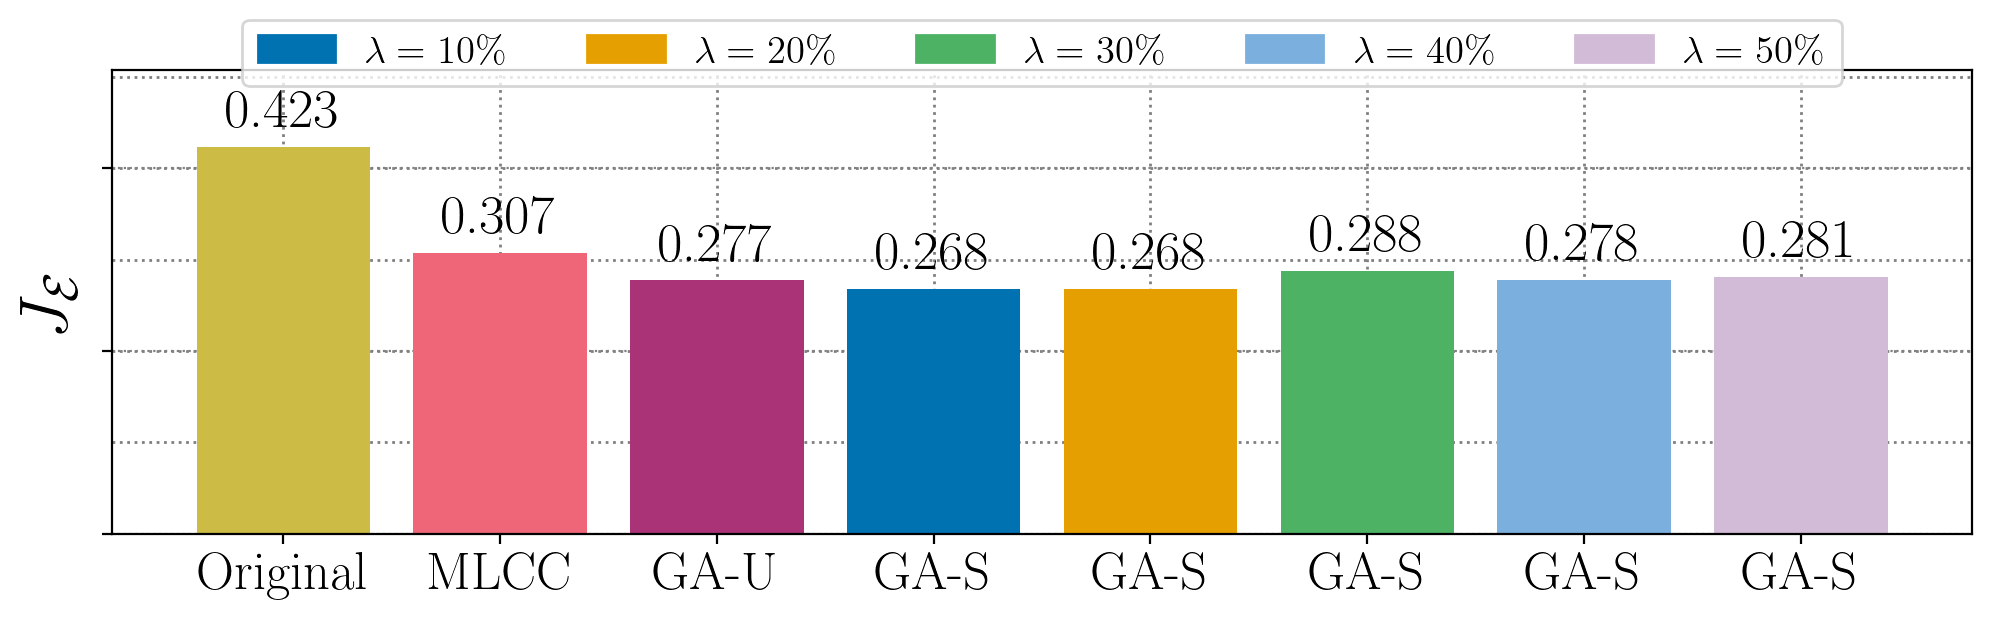
\includegraphics[width=\columnwidth]{Images/cyclist_exposure_3.png}
\caption{\footnotesize Cyclist exposure comparison of upper level $\mathbb{U}$ of Problem~1, where for \mbox{GA-S} the percentage indicates the $\lambda$ value for the threshold.}
\label{cyclist_exposure}
\end{figure}

Fig.~\ref{unfairness_result} presents the results of the sufficientarian approach in Problem~2, specifically to calculate the upper level $\mathbb{U}_{\text{thr}}$ for the different candidate solutions and threshold values given by  $\lambda$. We observe that when $\lambda$ is small, safety insufficiency remains low. However, as $\lambda$ increases, insufficiency also rises. Despite this, \mbox{GA-S} repeatedly achieves the greatest reduction in safety insufficiency.

% To better interpret these results, it is useful to compare them to a scenario where insufficiency is not explicitly optimized, such as in Problem~1, which focuses solely on minimizing cyclist exposure to traffic. Specifically, we consider $\mathbb{U}$ for this comparison. Fig.\ref{cyclist_exposure} shows the results for cyclist exposure, highlighting that \mbox{GA-U}  achieves the highest overall reduction in exposure. However, despite being designed to balance equity and exposure, \mbox{GA-S}  also performs similarly in minimizing traffic exposure across different threshold values. Since genetic algorithms provide locally optimal solutions rather than globally optimal ones, the specific outcome may vary depending on the problem instance. However, the comparable performance of \mbox{\mbox{GA-S} } suggests that incorporating fairness considerations into urban planning can effectively enhance cyclist safety without significantly compromising overall exposure reduction.
To better interpret these results, we compare them to a scenario where safety insufficiency is not explicitly addressed, as in Problem~1, which focuses solely on minimizing cyclist exposure to car traffic. Specifically, we consider the upper level $\mathbb{U}$ for this comparison. Fig.~\ref{cyclist_exposure} shows that \mbox{GA-U} achieves the greatest overall reduction in exposure. However, \mbox{GA-S} performs similarly across different thresholds, despite its being designed to balance insufficiency and exposure. Since genetic algorithms provide locally optimal solutions rather than globally optimal ones, the specific outcome may vary depending on the problem instance. However, the comparable performance of \mbox{\mbox{GA-S}} indicates that reduced insufficiency-oriented planning can enhance safety without substantially compromising overall exposure reduction.





\section{Conclusions and Future Work}
\label{conclusions}

% In this work, we integrated considerations from a transport justice perspective to ensure that the majority of individuals reached a minimum safety threshold within a quantitative optimization framework for cycling infrastructure planning. Using a bi-level approach, we balanced cyclist safety, comfort, and sufficientarian access to safe routes. Our findings showed that while MLCC enhanced connectivity and \mbox{\mbox{GA-U} } minimized overall cyclist exposure, \mbox{GA-S}  effectively reduces insufficiency safety while maintaining similar overall safety improvements. Moreover, the results suggested that incorporating transport justice considerations could enhance urban planning outcomes without compromising overall safety, highlighting the potential of justice-based principles in promoting fairer cycling infrastructure.





% This study serves as a first step toward incorporating transport justice-driven methodologies into cycling network optimization. Future work will extend this framework to a dynamic setting, analyzing how incremental infrastructure development influences safety, cyclist behavior, and car travel times \cite{mesbah2012bilevel}. This will allow us to evaluate the long term trade-offs between bicycle accessibility and motorized traffic efficiency, contributing to more adaptive and equitable transportation planning.

This work introduced a bi-level optimization framework that incorporates transport justice principles into cycling infrastructure planning. We balanced overall safety improvements with sufficientarian goals to ensure that most cyclists reach a minimum safety threshold.
Our results show that, compared to a conventional utilitarian approach, it is possible to significantly reduce safety insufficiency whilst still achieving similar overall safety improvements.
%Our results showed that while \mbox{\mbox{GA-U} } minimized overall exposure and MLCC enhanced connectivity, \mbox{GA-S}  effectively reduces safety insufficiency while maintaining similar overall safety improvements.
These findings highlight the value of integrating transport justice principles into infrastructure design.

Future work will extend this framework to a dynamic setting, analyzing how incremental infrastructure development influences safety, cyclist behavior, and car travel times \cite{mesbah2012bilevel}, supporting more equitable and adaptive transport planning.

% \section*{Acknowledgments}
% We thank Dr.\ I.\ New for proofreading this paper. M.\ Campero Jurado visited Eindhoven University of Technology with the support of an outgoing mobility grant IDEX from the Univ.\ Grenoble Alpes.

\section*{APPENDIX A}
\label{appendix:proof}

\begin{lemma}
The upper-level optimization problem $\mathbb{P}_{1}$ that minimizes cyclist exposure to traffic, given by the function
\begin{equation}
    \min_{\tilde{\mathbf{w}} \in \Omega} \; \mathbf{\mathcal{E}}(\tilde{\mathbf{w}})^\top\mathbf{x}(\tilde{\mathbf{w}})^{\star},
\end{equation}
where $\mathcal{E}_a(\tilde{w}_a) = d_a \cdot f_a(\tilde{w}_a)$ represents the traffic exposure factor, which depends on the DoS level $\tilde{w}_a$, is \textit{$i)$} non-linear and \textit{$ii)$} non-convex.
\end{lemma}

\textit{Proof of $i):$} The function $f_a(\tilde{w}_a)$ is piecewise constant, taking discrete values based on the DoS level $\tilde{w}_a$. This makes $f_a(\tilde{w}_a)$ inherently non-linear. The objective function $\mathbf{\mathcal{E}}(\tilde{\mathbf{w}})^\top\mathbf{x}(\tilde{\mathbf{w}})^{\star}$ is non-linear because
\begin{itemize}
    \item $f_a(\tilde{w}_a)$ is non-linear (piecewise constant), and
    \item the product $\mathcal{E}_a(\tilde{w}_a) = d_a \cdot f_a(\tilde{w}_a)$ introduces a non-linear dependence on $\tilde{\mathbf{w}}$.
\end{itemize}

\textit{Proof of $ii):$}
The feasible region $\Omega$ is defined by discrete DoS levels $\tilde{w}_a \in \{1, 2, 3, 4, 5, 6\}$. This set is finite and non-convex, as it does not form a continuous interval. The objective function is non-convex because
\begin{itemize}
    \item $f_a(\tilde{w}_a)$ is piecewise constant, and
    \item the product $\mathcal{E}_a(\tilde{w}_a) = d_a \cdot f_a(\tilde{w}_a)$ introduces non-convexity due to the discrete nature of $f_a(\tilde{w}_a)$.
\end{itemize}
Thus, the upper-level problem $\mathbb{U}$ is a mixed-integer non-linear program (MINLP) and is non-convex. \qedwhite

\begin{lemma}
    The lower-level problem $\mathbb{L}$ determines the cyclist flow distribution across the network using an AON traffic assignment model given by the objective function
    \begin{equation}
        \phi^{\tilde{\mathbf{w}}}(\mathbf{x}) = \sum_{a \in \mathcal{A}} b_{a}(\tilde{\mathbf{w}}) x_{a}
    \end{equation}
    is \textit{$i)$} linear and \textit{$ii)$} convex.
\end{lemma}

\textit{Proof of $i):$} 
For any constants $c_{1},c_{2} \in \mathbb{R}$, and flow vectors $\mathbf{x}, \hat{\mathbf{x}} \in \mathbb{R}^{|\mathcal{A}|}_{\geq 0}$, we have
\begin{align}
\phi^{\tilde{\mathbf{w}}}(c_{1}\mathbf{x} + c_{2}\bar{\mathbf{x}}) & = \sum_{a \in \mathcal{A}} b_{a}(\tilde{\mathbf{w}}) (c_{1}x_{a}+c_{2}\bar{x}_{a}) \\
% & = \sum_{a \in \mathcal{A}} (c_{1} b_{a}(\tilde{\mathbf{w}}) x_{a} + c_{2} b_{a}(\tilde{\mathbf{w}}) \bar{x}_{a}) \\ 
& = c_{1} \phi^{\tilde{\mathbf{w}}}(\mathbf{x}) + c_{2} \phi^{\tilde{\mathbf{w}}}(\mathbf{\bar{x}}),   
\end{align}
which implies that the function is linear.

\textit{Proof of $ii):$} It follows directly from $i)$, as the established linearity immediately implies convexity. Then, the feasible region, defined by linear flow conservation constraints, forms a convex polyhedron. As any convex combination of possible flows remains feasible, the lower-level problem is convex. The summary of the properties of the problems is given in Table~\ref{problem_properties} \qedwhite.
% For any $c \in \left [ 0,1\right ]$, and flow vectors $\mathbf{x}, \hat{\mathbf{x}}~\in~\mathbb{R}^{|\mathcal{A}|}_{\geq 0}$, we have
% \begin{equation}
%     \phi^{\tilde{\mathbf{w}}}(c \mathbf{x} + (1-c) \bar{\mathbf{x}}) = c  \phi^{\tilde{\mathbf{w}}}(\mathbf{x}) + (1-c)  \phi^{\tilde{\mathbf{w}}}(\mathbf{\bar{x}}).
% \end{equation}
% Since the inequality holds as an equality, the function is convex. 

\begin{table}[h!]
    \centering
    \begin{tabular}{l|c|c}
        \textbf{Property} & \textbf{$\mathbb{U}, \mathbb{U}_{\text{thr}}$: (DoS Selection)} & \textbf{$\mathbb{L}$: (AON Assignment)} \\ \hline
        Decision Variables & Discrete (\( \tilde{w}_a \)) & Continuous (\( x_a \)) \\
        Objective Function & Nonlinear & Linear \\
        Convexity & Non-convex & Convex \\
        Constraints & Discrete (DoS choices) & Linear flow conservation \\
        Complexity & NP-hard (MINLP) & Polynomial-time solvable \\
    \end{tabular}
    \caption{\footnotesize Comparison of upper- and lower-level problems properties.}
    \label{problem_properties}
\end{table}







\bibliographystyle{unsrt}
\bibliography{mybibfile}






\end{document}